%% bare_jrnl.tex
%% V1.3
%% 2007/01/11
%% by Michael Shell
%% see http://www.michaelshell.org/
%% for current contact information.
%%
%% This is a skeleton file demonstrating the use of IEEEtran.cls
%% (requires IEEEtran.cls version 1.7 or later) with an IEEE journal paper.
%%
%% Support sites:
%% http://www.michaelshell.org/tex/ieeetran/
%% http://www.ctan.org/tex-archive/macros/latex/contrib/IEEEtran/
%% and
%% http://www.ieee.org/



% *** Authors should verify (and, if needed, correct) their LaTeX system  ***
% *** with the testflow diagnostic prior to trusting their LaTeX platform ***
% *** with production work. IEEE's font choices can trigger bugs that do  ***
% *** not appear when using other class files.                            ***
% The testflow support page is at:
% http://www.michaelshell.org/tex/testflow/


%%*************************************************************************
%% Legal Notice:
%% This code is offered as-is without any warranty either expressed or
%% implied; without even the implied warranty of MERCHANTABILITY or
%% FITNESS FOR A PARTICULAR PURPOSE! 
%% User assumes all risk.
%% In no event shall IEEE or any contributor to this code be liable for
%% any damages or losses, including, but not limited to, incidental,
%% consequential, or any other damages, resulting from the use or misuse
%% of any information contained here.
%%
%% All comments are the opinions of their respective authors and are not
%% necessarily endorsed by the IEEE.
%%
%% This work is distributed under the LaTeX Project Public License (LPPL)
%% ( http://www.latex-project.org/ ) version 1.3, and may be freely used,
%% distributed and modified. A copy of the LPPL, version 1.3, is included
%% in the base LaTeX documentation of all distributions of LaTeX released
%% 2003/12/01 or later.
%% Retain all contribution notices and credits.
%% ** Modified files should be clearly indicated as such, including  **
%% ** renaming them and changing author support contact information. **
%%
%% File list of work: IEEEtran.cls, IEEEtran_HOWTO.pdf, bare_adv.tex,
%%                    bare_conf.tex, bare_jrnl.tex, bare_jrnl_compsoc.tex
%%*************************************************************************

% Note that the a4paper option is mainly intended so that authors in
% countries using A4 can easily print to A4 and see how their papers will
% look in print - the typesetting of the document will not typically be
% affected with changes in paper size (but the bottom and side margins will).
% Use the testflow package mentioned above to verify correct handling of
% both paper sizes by the user's LaTeX system.
%
% Also note that the "draftcls" or "draftclsnofoot", not "draft", option
% should be used if it is desired that the figures are to be displayed in
% draft mode.
%
\documentclass[journal]{IEEEtran}
\usepackage{blindtext}
\usepackage{graphicx}
\usepackage{longtable}
\usepackage{booktabs}
\usepackage[table,xcdraw]{xcolor}

% Some very useful LaTeX packages include:
% (uncomment the ones you want to load)


% *** MISC UTILITY PACKAGES ***
%
%\usepackage{ifpdf}
% Heiko Oberdiek's ifpdf.sty is very useful if you need conditional
% compilation based on whether the output is pdf or dvi.
% usage:
% \ifpdf
%   % pdf code
% \else
%   % dvi code
% \fi
% The latest version of ifpdf.sty can be obtained from:
% http://www.ctan.org/tex-archive/macros/latex/contrib/oberdiek/
% Also, note that IEEEtran.cls V1.7 and later provides a builtin
% \ifCLASSINFOpdf conditional that works the same way.
% When switching from latex to pdflatex and vice-versa, the compiler may
% have to be run twice to clear warning/error messages.






% *** CITATION PACKAGES ***
%
%\usepackage{cite}
% cite.sty was written by Donald Arseneau
% V1.6 and later of IEEEtran pre-defines the format of the cite.sty package
% \cite{} output to follow that of IEEE. Loading the cite package will
% result in citation numbers being automatically sorted and properly
% "compressed/ranged". e.g., [1], [9], [2], [7], [5], [6] without using
% cite.sty will become [1], [2], [5]--[7], [9] using cite.sty. cite.sty's
% \cite will automatically add leading space, if needed. Use cite.sty's
% noadjust option (cite.sty V3.8 and later) if you want to turn this off.
% cite.sty is already installed on most LaTeX systems. Be sure and use
% version 4.0 (2003-05-27) and later if using hyperref.sty. cite.sty does
% not currently provide for hyperlinked citations.
% The latest version can be obtained at:
% http://www.ctan.org/tex-archive/macros/latex/contrib/cite/
% The documentation is contained in the cite.sty file itself.






% *** GRAPHICS RELATED PACKAGES ***
%
\ifCLASSINFOpdf
  % \usepackage[pdftex]{graphicx}
  % declare the path(s) where your graphic files are
  % \graphicspath{{../pdf/}{../jpeg/}}
  % and their extensions so you won't have to specify these with
  % every instance of \includegraphics
  % \DeclareGraphicsExtensions{.pdf,.jpeg,.png}
\else
  % or other class option (dvipsone, dvipdf, if not using dvips). graphicx
  % will default to the driver specified in the system graphics.cfg if no
  % driver is specified.
  % \usepackage[dvips]{graphicx}
  % declare the path(s) where your graphic files are
  % \graphicspath{{../eps/}}
  % and their extensions so you won't have to specify these with
  % every instance of \includegraphics
  % \DeclareGraphicsExtensions{.eps}
\fi
% graphicx was written by David Carlisle and Sebastian Rahtz. It is
% required if you want graphics, photos, etc. graphicx.sty is already
% installed on most LaTeX systems. The latest version and documentation can
% be obtained at: 
% http://www.ctan.org/tex-archive/macros/latex/required/graphics/
% Another good source of documentation is "Using Imported Graphics in
% LaTeX2e" by Keith Reckdahl which can be found as epslatex.ps or
% epslatex.pdf at: http://www.ctan.org/tex-archive/info/
%
% latex, and pdflatex in dvi mode, support graphics in encapsulated
% postscript (.eps) format. pdflatex in pdf mode supports graphics
% in .pdf, .jpeg, .png and .mps (metapost) formats. Users should ensure
% that all non-photo figures use a vector format (.eps, .pdf, .mps) and
% not a bitmapped formats (.jpeg, .png). IEEE frowns on bitmapped formats
% which can result in "jaggedy"/blurry rendering of lines and letters as
% well as large increases in file sizes.
%
% You can find documentation about the pdfTeX application at:
% http://www.tug.org/applications/pdftex





% *** MATH PACKAGES ***
%
\usepackage[cmex10]{amsmath}
% A popular package from the American Mathematical Society that provides
% many useful and powerful commands for dealing with mathematics. If using
% it, be sure to load this package with the cmex10 option to ensure that
% only type 1 fonts will utilized at all point sizes. Without this option,
% it is possible that some math symbols, particularly those within
% footnotes, will be rendered in bitmap form which will result in a
% document that can not be IEEE Xplore compliant!
%
% Also, note that the amsmath package sets \interdisplaylinepenalty to 10000
% thus preventing page breaks from occurring within multiline equations. Use:
%\interdisplaylinepenalty=2500
% after loading amsmath to restore such page breaks as IEEEtran.cls normally
% does. amsmath.sty is already installed on most LaTeX systems. The latest
% version and documentation can be obtained at:
% http://www.ctan.org/tex-archive/macros/latex/required/amslatex/math/




% *** SPECIALIZED LIST PACKAGES ***
%
%\usepackage{algorithmic}
% algorithmic.sty was written by Peter Williams and Rogerio Brito.
% This package provides an algorithmic environment fo describing algorithms.
% You can use the algorithmic environment in-text or within a figure
% environment to provide for a floating algorithm. Do NOT use the algorithm
% floating environment provided by algorithm.sty (by the same authors) or
% algorithm2e.sty (by Christophe Fiorio) as IEEE does not use dedicated
% algorithm float types and packages that provide these will not provide
% correct IEEE style captions. The latest version and documentation of
% algorithmic.sty can be obtained at:
% http://www.ctan.org/tex-archive/macros/latex/contrib/algorithms/
% There is also a support site at:
% http://algorithms.berlios.de/index.html
% Also of interest may be the (relatively newer and more customizable)
% algorithmicx.sty package by Szasz Janos:
% http://www.ctan.org/tex-archive/macros/latex/contrib/algorithmicx/




% *** ALIGNMENT PACKAGES ***
%
%\usepackage{array}
% Frank Mittelbach's and David Carlisle's array.sty patches and improves
% the standard LaTeX2e array and tabular environments to provide better
% appearance and additional user controls. As the default LaTeX2e table
% generation code is lacking to the point of almost being broken with
% respect to the quality of the end results, all users are strongly
% advised to use an enhanced (at the very least that provided by array.sty)
% set of table tools. array.sty is already installed on most systems. The
% latest version and documentation can be obtained at:
% http://www.ctan.org/tex-archive/macros/latex/required/tools/


%\usepackage{mdwmath}
%\usepackage{mdwtab}
% Also highly recommended is Mark Wooding's extremely powerful MDW tools,
% especially mdwmath.sty and mdwtab.sty which are used to format equations
% and tables, respectively. The MDWtools set is already installed on most
% LaTeX systems. The lastest version and documentation is available at:
% http://www.ctan.org/tex-archive/macros/latex/contrib/mdwtools/


% IEEEtran contains the IEEEeqnarray family of commands that can be used to
% generate multiline equations as well as matrices, tables, etc., of high
% quality.


%\usepackage{eqparbox}
% Also of notable interest is Scott Pakin's eqparbox package for creating
% (automatically sized) equal width boxes - aka "natural width parboxes".
% Available at:
% http://www.ctan.org/tex-archive/macros/latex/contrib/eqparbox/





% *** SUBFIGURE PACKAGES ***
%\usepackage[tight,footnotesize]{subfigure}
% subfigure.sty was written by Steven Douglas Cochran. This package makes it
% easy to put subfigures in your figures. e.g., "Figure 1a and 1b". For IEEE
% work, it is a good idea to load it with the tight package option to reduce
% the amount of white space around the subfigures. subfigure.sty is already
% installed on most LaTeX systems. The latest version and documentation can
% be obtained at:
% http://www.ctan.org/tex-archive/obsolete/macros/latex/contrib/subfigure/
% subfigure.sty has been superceeded by subfig.sty.



%\usepackage[caption=false]{caption}
%\usepackage[font=footnotesize]{subfig}
% subfig.sty, also written by Steven Douglas Cochran, is the modern
% replacement for subfigure.sty. However, subfig.sty requires and
% automatically loads Axel Sommerfeldt's caption.sty which will override
% IEEEtran.cls handling of captions and this will result in nonIEEE style
% figure/table captions. To prevent this problem, be sure and preload
% caption.sty with its "caption=false" package option. This is will preserve
% IEEEtran.cls handing of captions. Version 1.3 (2005/06/28) and later 
% (recommended due to many improvements over 1.2) of subfig.sty supports
% the caption=false option directly:
%\usepackage[caption=false,font=footnotesize]{subfig}
%
% The latest version and documentation can be obtained at:
% http://www.ctan.org/tex-archive/macros/latex/contrib/subfig/
% The latest version and documentation of caption.sty can be obtained at:
% http://www.ctan.org/tex-archive/macros/latex/contrib/caption/




% *** FLOAT PACKAGES ***
%
%\usepackage{fixltx2e}
% fixltx2e, the successor to the earlier fix2col.sty, was written by
% Frank Mittelbach and David Carlisle. This package corrects a few problems
% in the LaTeX2e kernel, the most notable of which is that in current
% LaTeX2e releases, the ordering of single and double column floats is not
% guaranteed to be preserved. Thus, an unpatched LaTeX2e can allow a
% single column figure to be placed prior to an earlier double column
% figure. The latest version and documentation can be found at:
% http://www.ctan.org/tex-archive/macros/latex/base/



%\usepackage{stfloats}
% stfloats.sty was written by Sigitas Tolusis. This package gives LaTeX2e
% the ability to do double column floats at the bottom of the page as well
% as the top. (e.g., "\begin{figure*}[!b]" is not normally possible in
% LaTeX2e). It also provides a command:
%\fnbelowfloat
% to enable the placement of footnotes below bottom floats (the standard
% LaTeX2e kernel puts them above bottom floats). This is an invasive package
% which rewrites many portions of the LaTeX2e float routines. It may not work
% with other packages that modify the LaTeX2e float routines. The latest
% version and documentation can be obtained at:
% http://www.ctan.org/tex-archive/macros/latex/contrib/sttools/
% Documentation is contained in the stfloats.sty comments as well as in the
% presfull.pdf file. Do not use the stfloats baselinefloat ability as IEEE
% does not allow \baselineskip to stretch. Authors submitting work to the
% IEEE should note that IEEE rarely uses double column equations and
% that authors should try to avoid such use. Do not be tempted to use the
% cuted.sty or midfloat.sty packages (also by Sigitas Tolusis) as IEEE does
% not format its papers in such ways.


%\ifCLASSOPTIONcaptionsoff
%  \usepackage[nomarkers]{endfloat}
% \let\MYoriglatexcaption\caption
% \renewcommand{\caption}[2][\relax]{\MYoriglatexcaption[#2]{#2}}
%\fi
% endfloat.sty was written by James Darrell McCauley and Jeff Goldberg.
% This package may be useful when used in conjunction with IEEEtran.cls'
% captionsoff option. Some IEEE journals/societies require that submissions
% have lists of figures/tables at the end of the paper and that
% figures/tables without any captions are placed on a page by themselves at
% the end of the document. If needed, the draftcls IEEEtran class option or
% \CLASSINPUTbaselinestretch interface can be used to increase the line
% spacing as well. Be sure and use the nomarkers option of endfloat to
% prevent endfloat from "marking" where the figures would have been placed
% in the text. The two hack lines of code above are a slight modification of
% that suggested by in the endfloat docs (section 8.3.1) to ensure that
% the full captions always appear in the list of figures/tables - even if
% the user used the short optional argument of \caption[]{}.
% IEEE papers do not typically make use of \caption[]'s optional argument,
% so this should not be an issue. A similar trick can be used to disable
% captions of packages such as subfig.sty that lack options to turn off
% the subcaptions:
% For subfig.sty:
% \let\MYorigsubfloat\subfloat
% \renewcommand{\subfloat}[2][\relax]{\MYorigsubfloat[]{#2}}
% For subfigure.sty:
% \let\MYorigsubfigure\subfigure
% \renewcommand{\subfigure}[2][\relax]{\MYorigsubfigure[]{#2}}
% However, the above trick will not work if both optional arguments of
% the \subfloat/subfig command are used. Furthermore, there needs to be a
% description of each subfigure *somewhere* and endfloat does not add
% subfigure captions to its list of figures. Thus, the best approach is to
% avoid the use of subfigure captions (many IEEE journals avoid them anyway)
% and instead reference/explain all the subfigures within the main caption.
% The latest version of endfloat.sty and its documentation can obtained at:
% http://www.ctan.org/tex-archive/macros/latex/contrib/endfloat/
%
% The IEEEtran \ifCLASSOPTIONcaptionsoff conditional can also be used
% later in the document, say, to conditionally put the References on a 
% page by themselves.


\usepackage{pdfpages}


% *** PDF, URL AND HYPERLINK PACKAGES ***
%
\usepackage{url}
\usepackage{hyperref}
% url.sty was written by Donald Arseneau. It provides better support for
% handling and breaking URLs. url.sty is already installed on most LaTeX
% systems. The latest version can be obtained at:
% http://www.ctan.org/tex-archive/macros/latex/contrib/misc/
% Read the url.sty source comments for usage information. Basically,
% \url{my_url_here}.





% *** Do not adjust lengths that control margins, column widths, etc. ***
% *** Do not use packages that alter fonts (such as pslatex).         ***
% There should be no need to do such things with IEEEtran.cls V1.6 and later.
% (Unless specifically asked to do so by the journal or conference you plan
% to submit to, of course. )


% correct bad hyphenation here
\hyphenation{op-tical net-works semi-conduc-tor}


\begin{document}
%
% paper title
% can use linebreaks \\ within to get better formatting as desired
\title{Predicting Myers-Briggs Type Indicator From Written Texts Using Supervised Learning}

% author names and IEEE memberships
% note positions of commas and nonbreaking spaces ( ~ ) LaTeX will not break
% a structure at a ~ so this keeps an author's name from being broken across
% two lines.
% use \thanks{} to gain access to the first footnote area
% a separate \thanks must be used for each paragraph as LaTeX2e's \thanks
% was not built to handle multiple paragraphs
%

\author{Linus~Kortesalmi,~linko538@student.liu.se}%~\IEEEmembership{Member,~IEEE,}
       %John~Doe,~\IEEEmembership{Fellow,~OSA,}
        %and~Jane~Doe,~\IEEEmembership{Life~Fellow,~IEEE}% <-this % stops a space
%\thanks{M. Shell is with the Department
%of Electrical and Computer Engineering, Georgia Institute of %Technology, Atlanta,
%GA, 30332 USA e-mail: (see http://www.michaelshell.org/contact.html).}% <-this % stops a space
%\thanks{J. Doe and J. Doe are with Anonymous University.}% <-this % stops a space
%\thanks{Manuscript received April 19, 2005; revised January 11, 2007.}}

% note the % following the last \IEEEmembership and also \thanks - 
% these prevent an unwanted space from occurring between the last author name
% and the end of the author line. i.e., if you had this:
% 
% \author{....lastname \thanks{...} \thanks{...} }
%                     ^------------^------------^----Do not want these spaces!
%
% a space would be appended to the last name and could cause every name on that
% line to be shifted left slightly. This is one of those "LaTeX things". For
% instance, "\textbf{A} \textbf{B}" will typeset as "A B" not "AB". To get
% "AB" then you have to do: "\textbf{A}\textbf{B}"
% \thanks is no different in this regard, so shield the last } of each \thanks
% that ends a line with a % and do not let a space in before the next \thanks.
% Spaces after \IEEEmembership other than the last one are OK (and needed) as
% you are supposed to have spaces between the names. For what it is worth,
% this is a minor point as most people would not even notice if the said evil
% space somehow managed to creep in.



% The paper headers
%\markboth{Journal of \LaTeX\ Class Files,~Vol.~6, No.~1, January~2007}%
%{Shell \MakeLowercase{\textit{et al.}}: Bare Demo of IEEEtran.cls for Journals}
% The only time the second header will appear is for the odd numbered pages
% after the title page when using the twoside option.
% 
% *** Note that you probably will NOT want to include the author's ***
% *** name in the headers of peer review papers.                   ***
% You can use \ifCLASSOPTIONpeerreview for conditional compilation here if
% you desire.




% If you want to put a publisher's ID mark on the page you can do it like
% this:
%\IEEEpubid{0000--0000/00\$00.00~\copyright~2007 IEEE}
% Remember, if you use this you must call \IEEEpubidadjcol in the second
% column for its text to clear the IEEEpubid mark.



% use for special paper notices
%\IEEEspecialpapernotice{(Invited Paper)}




% make the title area
\maketitle
% IEEEtran.cls defaults to using nonbold math in the Abstract.
% This preserves the distinction between vectors and scalars. However,
% if the journal you are submitting to favors bold math in the abstract,
% then you can use LaTeX's standard command \boldmath at the very start
% of the abstract to achieve this. Many IEEE journals frown on math
% in the abstract anyway.
\begin{abstract}
    This work experiments with supervised learning classifiers to predict the Myers-Briggs type of a user based on written text.
    The models are tested with features extracted from the latent Dirichlet allocation model, the TF-IDF model and the bag-of-letters model.
    The Gradient Boosting Classifier is shown to achieve the best performance with a test accuracy of 30.3\%.
    Improvements to the classifiers are proposed and the limitations of the data set are discussed.
\end{abstract}

% Note that keywords are not normally used for peerreview papers.
%\begin{IEEEkeywords}
%Natural Language Processing, Classification, Psychology, MBTI.
%\end{IEEEkeywords}






% For peer review papers, you can put extra information on the cover
% page as needed:
% \ifCLASSOPTIONpeerreview
% \begin{center} \bfseries EDICS Category: 3-BBND \end{center}
% \fi
%
% For peerreview papers, this IEEEtran command inserts a page break and
% creates the second title. It will be ignored for other modes.
\IEEEpeerreviewmaketitle

\section{Introduction}

The Myers-Briggs Type Indicator has under the past few years come under heavy criticism \cite{pittenger1993, grant-mbti, rose-mbti, bbc-mbti, winkie-mbti}.
However, it is still a popular \cite{MBTI-trend} personality trait indicator.
This work aims to explore if text written by an individual can be used to predict the Myers-Briggs type for that individual.
It uses Natural Language Processing (NLP) techniques and supervised learning methods.
Section \ref{sec:theory} briefly explains the Myers-Briggs Type Indicator, common NLP techniques and machine learning models used.
Related work is presented in Section \ref{sec:related-work}.
The method is covered in Section \ref{sec:method} and the results from the method is presented in Section \ref{sec:results} and Appendix \ref{appendix:results}.
The results and limitations in the work are discussed in Section \ref{sec:discussion}.
The conclusions from this work are present in Section \ref{sec:conclusion} and potential future work is discussed in Section \ref{sec:future-work}.

\section{Theory} \label{sec:theory}

This section will briefly cover the basics of Myers-Briggs Type Indicator, language modelling, feature representations, common supervised learning models and evaluation metrics.

\subsection{Myers-Briggs Type Indicator}
The foundation of the Myers-Briggs Type Indicator (MBTI) is derived from the work of Carl G. Jung \cite{jung2014psychological}.
The idea behind MBTI was to make the concepts observed by Jung more accessible to the public \cite{mbti}.
Table \ref{tab:mbti-types} contains the 16 personality types defined by Myers-Briggs \cite{mbti}.

\subsubsection{Introversion and Extroversion}
Introversion (I) and extroversion (E) is used to describe what an individual focuses on and draws their energy from.
Introversion means that the individual focuses on his/her own "world", which means that they draw energy from ideas and memories and from self-reflection \cite{mbti-IE}.
Extroversion is the opposite side; energy is drawn from activities and events with others \cite{mbti-IE}.
Problems for people with the extroversion type are typically solved by talking and discussing with others out loud \cite{mbti-IE}.

\subsubsection{Intuition and Sensing}
Intuition (N) and sensing (S) describes how individuals handles information.
Intuition means that individuals pay more attention to patterns, impressions, theoretical concepts and abstract theories \cite{mbti-NS}.
Sensing is, on the other hand, connected to the five senses.
Information is gathered from the physical connection to the world, e.g., what you hear, smell and touch \cite{mbti-NS}.

\subsubsection{Thinking and Feeling}
Thinking (T) and feeling (F) covers how individuals perform decision making.
Individuals with the thinking type typically analyse ground truths and use logical reasoning to make a decision; pros and cons are analysed \cite{mbti-TF}.
The feeling type describes people who take the opinion of others into consideration \cite{mbti-TF}.
They weigh the outcome of the situation and try to maintain harmony, by caring about the point-of-view of others \cite{mbti-TF}.

\subsubsection{Judging and Perceiving}
Judging (J) and perceiving (P) is the final pair of the MBTI.
This pair is related to how others typically see you.
People with the judging trait usually live more structured lives than those with the perceiving trait \cite{mbti-JP}.
The major difference between this pair and the pairs covered before is that this trait is based on the side individuals let others see \cite{mbti-JP}.
For example, an individual can be structured and live ordered lives when alone, but in the interaction with others they tend to be interpreted as spontaneous and open-ended \cite{mbti-JP}.

\begin{table}[!t]
    %% increase table row spacing, adjust to taste
    \renewcommand{\arraystretch}{3}
    % if using array.sty, it might be a good idea to tweak the value of
    % \extrarowheight as needed to properly center the text within the cells
    \caption{Myers-Briggs Type Indicator Table}
    \label{tab:mbti-types}
    \centering
    %% Some packages, such as MDW tools, offer better commands for making tables
    %% than the plain LaTeX2e tabular which is used here.
    \begin{tabular}{|c|c|c|c|}
        \hline
        ISTJ & ISFJ & INFJ & INTJ \\
        \hline
        ISTP & ISFP & INFP & INTP \\
        \hline
        ESTP & ESFP & ENFP & ENTP \\
        \hline
        ESTJ & ESFJ & ENFJ & ENTJ \\
        \hline
    \end{tabular}
\end{table}

\subsection{Document Representation}
A document $d_i$ can be mathematically represented as a vector $d_i = (w_1, \ldots, w_N)$, where $w_i$ is the $i$-th word (term) in the document.
The words (terms) could, for example, be unigrams (Section \ref{sec:theory-bow}), bigrams (Section \ref{sec:theory-bigram}) or letters (Section \ref{sec:theory-letters}).

\subsection{Latent Dirichlet Allocation}
The latent Dirichlet allocation (LDA) model produces top topic terms for each topic in the model.
It can also be used to calculate the topic distribution for a document.

The LDA model, described by Blei et al. in \cite{Blei2003}, is a probabilistic generative model built on the notion of underlying topics.
A document can belong to several topics simultaneously (with a probability $p(\alpha_i)$ of belonging to topic $\alpha_i$).
All the terms in a collection can belong to their own topic(s).
Each term in a document in a corpus is assumed to be generated from a topic (following a multinomial distribution with a latent parameter drawn from a Dirichlet distribution).
The LDA model can thus for a given document calculate the probability of that document belonging to some topic $\alpha_i$.

\subsection{Features} \label{sec:theory-features}

\subsubsection{Normalisation}
Normalisation transforms the data values above $0$ in the feature vector to be in the range $(0, 1]$.

\subsubsection{Bag-Of-Words} \label{sec:theory-bow}
The bag-of-words model is a simple representation of a document.
The model ignores the order of words and the words occurring before the $i$-th word ($w_i$):

\begin{equation*}
    p(w_i|w_1, \ldots, w_{i-1}) = p(w_i)
\end{equation*}

The feature vector consists of occurrence counts of words in a dictionary, where each word is represented by an index in the vector.
The dictionary can either be predefined or created from the training set.
One limitation of the bag-of-words model is how to handle words not present in the training corpus.
Unknown words can either be discarded or replaced with an \emph{UNK} tag.
The count vector can then be normalised, smoothed or used as-is.

\subsubsection{TF-IDF}
Term frequency and inverted document frequency (TF-IDF) can be constructed from a bag-of-words model.
The TF is the word (term) counts for a document (typically normalised) and the IDF is the document frequency for that word

\begin{equation*} \label{eq:idf}
    IDF_{k_i} = log(N / n_i)
\end{equation*}
where $N$ is the number of documents and $n_i$ is the number of documents where term $k_i$ appears.

\subsubsection{Bigram Model} \label{sec:theory-bigram}
The bigram model is similar to the bag-of-words model in Section \ref{sec:theory-bow}.
Instead of using counts of single words the bigram model uses pairs of adjacent words as features:

\begin{equation*}
    p(w_i|w_1, \ldots, w_{i-1}) = p(w_i|w_{i-1})
\end{equation*}

The appearance order for different pairs is ignored after construction; it is only the counts of pairs that are interesting.

\subsubsection{Bag-Of-Letters} \label{sec:theory-letters}
The bag-of-letters feature vector is a simplified variant of the Bag-of-words model.
The features are constructed from a predefined alphabet consisting of letters and characters.
Similar to the bag-of-words model, the symbols in the alphabet are counted for each document.
The feature vector can then be normalised or used as-is.

\subsubsection{Topic Distribution (TD)}
The LDA model can calculate the probability distribution $$T_{d_i}=[p(\alpha_1),\ldots,p(\alpha_t)]$$ over all $t$ topics ($\alpha_1,\ldots,\alpha_t$) for a given document $d_i$.
$p(\alpha_i)$ is the probability that document $d_i$ belongs to topic $\alpha_i$.
The distribution can thus be used to determine which topic(s) the document was generated from.
This probability distribution can be directly used as a feature vector for various models.

\subsubsection{Topic Terms (TT)} \label{sec:theory-topic-terms}
In \cite{Chen2016}, Chen et al. try to use LDA to improve the performance of Support Vector Machines for text classification.
In their work they combine the topic distribution of a document from a LDA model together with the top terms for the topics.
The same approach is tested in this work.
The topic terms feature vectors are constructed by first calculating the topic distribution $T_{d_i}$ for each document $d_i$.
Then, for each topic $\alpha_i$, the $n$ top topic terms ($\beta_{i, 1}, \ldots, \beta_{i, n}$) are used to construct the feature vector.
The topic distribution and the topic terms can be retrieved from a LDA model with $t$ topics.
The feature vector $f_{d_i}$ for a document $d_i$  is thus defined by 
\begin{equation*}
    f_{d_i}=[\beta_1, \ldots, \beta_t]
\end{equation*}
where $\beta_i$ is short-hand notation for the values $\beta_{i, 1}, \ldots, \beta_{i, n}$. 
The dimension of a topic terms feature vector for one document is $t*n$ feature values.
Each value in the feature vector is initialised to zero.

The topic distribution determines how many top topic terms shall be counted from each topic in the LDA model.
If topic $\alpha_i$  has probability $p_i$, then the number of top topic terms to be used ($n_i$) from topic $\alpha_i$ is given by Equation \ref{eq:n-top-topic-terms}.

\begin{equation} \label{eq:n-top-topic-terms}
    n_i=Round(p_i*n)
\end{equation}

The $n-n_i$ top terms not used in topic $\alpha_i$ have their feature values set to zero.
The feature value for each of the $n_i$ top terms is set according to Equation \ref{eq:feature-value}.

\begin{equation} \label{eq:feature-value}
    feature\ value =\left\{
                \begin{array}{ll}
                  1+TF, \quad \ if\ term\ present\\
                  1, \qquad\qquad otherwise
                \end{array}
              \right.
\end{equation}

If the term is present in document $d_i$ it is counted and the feature value is set to $1+TF$.
$TF$  is the number of times the term occurs in document $d_i$.  
If the term is not in the document, the feature value for the term is set to $1$.
If a document $d_i$  is calculated by the LDA to belong to a topic $\alpha_i$, then Equation \ref{eq:feature-value} would give more weight to the top terms that do occur in $d_i$, compared to the missing ones.

For example, a LDA with five topics ($t=5$) and a document $d_i$  with the topic distribution 
\[T_{d_i}=[0.01, 0.15, 0.75, 0.09, 0]\]
and $n=10$ top topic terms would result in a feature vector $f_{d_i}$ where:

\begin{itemize}
    \item $n_1$ is rounded down to zero, thus setting all values for the 10 top topic terms in $\alpha_1$ to zero.
    \item $n_2$ is rounded up to two, which means that only the values for the two top terms in $\alpha_2$ are updated to $1+TF$.
    \item $n_3$  is rounded up to 8, which means the values for the 8 top terms in topic $\alpha_3$ are updated.
    \item $n_4$ is rounded up to one, which means that only the value for the top term in topic $\alpha_4$ is updated.
    \item $n_5$  is zero, thus all 10 values are set to zero (same as $n_1$).
\end{itemize}

\subsection{Models} \label{sec:theory-models}

Various supervised models can be used for classification.
This section will very briefly cover the models used in this work.

\subsubsection{Linear Support Vector Classification}
The linear Support Vector Classifier (LinSVC) can efficiently handle sparse features\footnote{http://scikit-learn.org/stable/modules/generated/sklearn.svm.LinearSVC.html}.
The SVC has a slightly different mathematical formulation than the traditional Support Vector Machine (SVM), but the idea behind the model is the same as in the SVM case.
A hyperplane is constructed in order to try and separate the different classes with as big of a margin as possible.
The margin is defined as the distance from the hyperplane to the nearest point.
Slack can be introduced in order to allow for misclassifications, as needed in the case of data not being linearly separable.
Regularisation is typically used in order to control the slack, otherwise the margin would be maximised by potentially misclassifying all data points.

\subsubsection{Logistic Regression Classifier}
The Logistic Regression (LR) classifier, also called logit or MaxEnt, is a probabilistic classifier consisting of linear combinations of predictor functions and weights.
The predictor function calculates the probability of a data point $X_i$ belonging to a class $K_i$ ($p(K_i|X_i)$), divided by the probability that it belongs to all other classes ($p(\{K \setminus K_i\} | X_i)$).

\subsubsection{Extra Trees Classifier}
The Extra Trees (ET) classifier is a variant of the well-known Random Forest (RF) classifier.
Instead of choosing the best decision boundary at each split it continuously chooses attributes and cut-points at random \cite{Geurts2006}.
It can be heavily tuned to the problem at hand with various parameters \cite{Geurts2006}.

\subsubsection{AdaBoost Classifier}
The AdaBoost (AB) classifier is an ensemble method which combines multiple weak learners (estimators) \cite{Freund1995}.
The later weak learners in the chain are tweaked in order to solve those samples that were misclassified by the previous learners \cite{Freund1995}.
The result of each weak learner is combined into a weighted sum \cite{Freund1995}.

\subsubsection{Gradient Boosting Classifier}
The Gradient Boosting (GB) classifier is a variant of the AdaBoost classifier.
If the exponential loss function is used, then it turns into the AdaBoost classifier.
The model creates multiple decision trees that are, in each iterative stage, fitted with the negative gradient of the multinomial deviance loss function.

\subsection{Exploratory Data Analysis}
Exploratory data analysis (EDA) is a broad concept containing various techniques \cite{Hoaglin2003, Tukey1977, Velleman1981} that can be used to explore and analyse data.
Some early techniques include stem-and-leaf plots and box plots.
EDA can be seen as applying tools and statistics in a meaningful way.
It could, for example, be used to perform variance analysis, detect outliers or smooth the data \cite{Hoaglin2003, Tukey1977, Velleman1981}.

\subsubsection{Word clouds}
In the field of NLP, the use of word clouds can help visualise important aspects of the data.
Word clouds are generated by simply counting the occurrence of each word in the data set and presenting the most common words in an image.
The most frequent words are typically presented with a larger font.

\subsection{Evaluation Metrics} \label{sec:evaluation-metrics}
Common evaluation metrics in the NLP field are Accuracy (Equation \ref{eq:accuracy}), Precision (Equation \ref{eq:precision}), Recall (Equation \ref{eq:recall}) and F1 Score (Equation \ref{eq:f1-score}).
They are computed by calculating the number of True Positives (TP), True Negatives (TN), False Positives (FP) and False Negatives (FN).

\begin{equation} \label{eq:accuracy}
    Accuracy = \frac{TP + TN}{TP + TN + FP + FN}
\end{equation}

\begin{equation} \label{eq:precision}
    Precision = \frac{TP}{TP + FP}
\end{equation}

\begin{equation} \label{eq:recall}
    Recall = \frac{TP}{TP + FN}
\end{equation}

\begin{equation} \label{eq:f1-score}
    F1\ Score = \frac{2 * Recall * Precision}{Recall + Precision}
\end{equation}


\section{Related Work}

In \cite{maneural}, Ma et al. train Neural Networks (NNs) to predict Myers-Briggs personality types based on the writing style.
The data used in \cite{maneural} was manually crafted by generating a mapping between famous authors and their MBTI.
The text in books written by the authors were then retrieved and used in the work.
The best accuracy obtained by Ma et al. was 37\%, using a Recurrent NN with long short-term memory (LSTM).

\section{Method} \label{sec:method}

This section covers the data set used in this work and the preprocessing and feature extraction used.
The implementations of the classification models used are briefly mentioned.
The work was implemented using Python\footnote{https://www.python.org/} version 3.6.2.
\subsection{Data Set}
The data set used in this work was downloaded from Kaggle\footnote{https://www.kaggle.com/}.
It contains data from 8675 Personality Cafe \footnote{http://personalitycafe.com/forum/} forum users.
Each data entry contains the 50 latest posts from a user, together with the MBTI of the user.
30\% of the data was used as a test set and the training set consisted of the remaining 70\%.
\subsection{Exploratory Data Analysis}
A simple EDA was performed to better understand the data.
This work mainly used word clouds, bar plots and document content analysis.

\subsubsection{Word clouds}
The Python library \texttt{word\_cloud}\footnote{https://github.com/amueller/word\_cloud} was used to generate word clouds.
First a word cloud was generated from all the documents in the data set.
The idea behind this general word cloud was to see if there were any terms or topics that needed further investigation.
After the general word cloud was generated the documents were partitioned on their respective MBTI labels.
A word cloud was then generated for each MBTI label.
Appendix \ref{sec:wordclouds} contains all the word clouds generated.

\subsection{Preprocessing} \label{sec:method-preprocessing} 
The data set was preprocessed according to the following steps:

\subsubsection{Standardising}
The data set was standardised so that any leading or trailing "\texttt{'}" characters were removed.

\subsubsection{Tagging}
All URLs in the data set were replaced with a \texttt{<URL>} tag.
Only URLs were replaced with a tag in this work.

\subsubsection{Tokenising}
The data was tokenised using the tokeniser from the \texttt{NLTK}\footnote{http://www.nltk.org/} package.
The \texttt{NLTK} package also contains an English stop word list that were used to remove stop words.

\subsubsection{Stemming}
The Snowball stemmer from the \texttt{NLTK} package was used to stem the tokens in the preprocessing step. 

\subsection{Features}

The features covered in Section \ref{sec:theory-features} were extracted and tested with the models in Section \ref{sec:theory-models}.
This section covers the implementation-specific details for the feature extraction used in this work.

\subsubsection{Filter Levels} \label{sec:method-filter-levels}
Three \emph{filter levels} were introduced in order to try and improve the quality of the different feature models:

\paragraph{Normal Filter} \label{sec:method-normal-filter}
This filter level only applies the first two steps in the preprocessing mentioned in Section \ref{sec:method-preprocessing}.

\paragraph{Type Filter} \label{sec:method-type-filter}
This filter level applies the standard preprocessing, but it also removes any MBTIs found in the data set.
The filtering is done by adding the MBTIs to the stop-word list.

\paragraph{Extreme Filter} \label{sec:method-extreme-filter}
This filter level applies both the standard preprocessing and the removal of MBTIs, as in the case of the Type Filter.
It also removes any tokens that occur in less than five documents or in more than 50\% of the documents.

\subsubsection{Latent Dirichlet Allocation}
The library \texttt{gensim}\footnote{https://radimrehurek.com/gensim/} was used to implement the LDA model.
Six LDA models with 10, 16, 25, 50, 75 and 100 topics were trained for each filter level.
The LDA models were used to extract the topic terms and topic distribution feature vectors covered in Section \ref{sec:theory-features}.


\subsubsection{Topic Terms Feature Vector}
The topic term feature vector covered in Section \ref{sec:theory-topic-terms} was implemented using 10 topic terms.
The feature vector was normalised for the LinSVC, GB and ET classifiers.


\subsection{Model Implementation and Training}
The models used the implementations in the \texttt{scikit-learn}\footnote{http://scikit-learn.org/stable/} package for Python.
The main parameters for each model was tuned using the \texttt{GridSearchCV} class, which allows a grid of parameter values to be tested for each model using cross-validation. 
The cross-validation used in this work was \texttt{StratifiedKFold} using five folds.
The stratified $k$-folds tries to maintain the imbalance of the data set in the different folds. 
The \texttt{F1\_micro} score was used to choose the best cross-validated model during the \texttt{GridSearchCV} parameter tuning.
The micro score globally counts all TPs, TNs, FPs and FNs, which is more suitable if the data set is imbalanced. 

\subsubsection{Initial Models} \label{sec:method-initial-models}
The first part was to use only the standardised and tagged data set (see Section \ref{sec:method-normal-filter}) in a LR model.
The classifier was tested using the bag-of-words model, the bigram model and the TF-IDF model.
The best LR model obtained through the \texttt{GridSearchCV} process was then evaluated on the test set.

The next step was to try the ET classifier on the standardised and tagged data set.
The features were extracted by using TF-IDF with a unigram model, followed by truncated Singular Value Decomposition (SVD) to reduce the number of features.
\texttt{GridSearchCV} was used to optimise the parameters for TF-IDF, truncated SVD and the ET classifier.

\subsubsection{Type Filter Models} \label{sec:method-type-filter-models}
The second part was to filter out the MBTIs from the data set, see Section \ref{sec:method-type-filter}.
Instead of using the built-in tokenisation methods in \texttt{scikit-learn}, a custom corpus was built using the \texttt{NLTK} library.
All the models briefly covered in Section \ref{sec:theory-models} were used on the type-filtered data set.
The parameters for each model was individually optimised using \texttt{GridSearchCV}.

\subsubsection{Extreme Filter Models}  \label{sec:method-extreme-filter-models}
The final part was to also filter out extreme words from the data set, see Section \ref{sec:method-extreme-filter}.
The same models are used as in Section \ref{sec:method-type-filter-models}.
The parameters were again optimised using \texttt{GridSearchCV}.
\section{Type Filter and Extreme Filter Results} \label{appendix:results}
This appendix contains the results from using the implemented models on data with different filter levels (see Section \ref{sec:method-filter-levels}).
Table \ref{tab:results-types} and Table \ref{tab:results-extremes} contain the results from using the Type Filter (Section \ref{sec:method-type-filter}) and the Extreme Filter (Section \ref{sec:method-extreme-filter}), respectively.
\clearpage

% Please add the following required packages to your document preamble:
% If you use beamer only pass "xcolor=table" option, i.e. \documentclass[xcolor=table]{beamer}
  \begin{table}[]
    \centering
    \caption{Results from Type filtering}
    \label{tab:results-types}
    \begin{tabular}{@{}llllllllll@{}}
    \toprule
    \rowcolor[HTML]{FFFFFF} 
    \textbf{Normalized} & \textbf{Topics} & \textbf{Filter Level} & \textbf{Feature Type} & \textbf{Model}      & \textbf{Train Accuracy} & \textbf{Test Accuracy} & \textbf{Precision} & \textbf{Recall} & \textbf{F1 Score} \\ \midrule
    No                  & -               & Types                 & Characters            & Linear SVC          & 0.2621870882740448      & 0.26930464848252017    & 0.19               & 0.27            & 0.20              \\
    No                  & -               & Types                 & Characters            & Logistic Regression & 0.11495388669301712     & 0.1260084517864003     & 0.25               & 0.13            & 0.16              \\
    Yes                 & -               & Types                 & Characters            & Extra Trees         & 0.2439064558629776      & 0.24587014982712255    & 0.16               & 0.25            & 0.17              \\
    No                  & -               & Types                 & Characters            & AdaBoost            & 0.22266139657444006     & 0.2155205532078371     & 0.21               & 0.22            & 0.13              \\
    Yes                 & -               & Types                 & Characters            & GradBoost           & 0.24769433465085638     & 0.2397233960814445     & 0.17               & 0.24            & 0.18              \\
    -                   & 100             & Types                 & Topic Distribution    & Linear SVC          & 0.2887022397891963      & 0.27276219746446406    & 0.28               & 0.27            & 0.20              \\
    -                   & 100             & Types                 & Topic Distribution    & Logistic Regression & 0.13554018445322794     & 0.13753361505954667    & 0.25               & 0.14            & 0.15              \\
    -                   & 100             & Types                 & Topic Distribution    & Extra Trees         & 0.25148221343873517     & 0.24433346139070303    & 0.21               & 0.24            & 0.21              \\
    -                   & 100             & Types                 & Topic Distribution    & AdaBoost            & 0.255764163372859       & 0.2535535920092201     & 0.17               & 0.25            & 0.14              \\
    -                   & 100             & Types                 & Topic Distribution    & GradBoost           & 0.28573781291172595     & 0.27276219746446406    & 0.21               & 0.27            & 0.22              \\
    -                   & 75              & Types                 & Topic Distribution    & Linear SVC          & 0.26515151515151514     & 0.26661544371878604    & 0.19               & 0.27            & 0.20              \\
    -                   & 75              & Types                 & Topic Distribution    & Logistic Regression & 0.10013175230566534     & 0.11025739531310026    & 0.28               & 0.11            & 0.13              \\
    -                   & 75              & Types                 & Topic Distribution    & Extra Trees         & 0.22990777338603424     & 0.2320399538993469     & 0.19               & 0.23            & 0.20              \\
    -                   & 75              & Types                 & Topic Distribution    & AdaBoost            & 0.2524703557312253      & 0.2451018056089128     & 0.15               & 0.25            & 0.15              \\
    -                   & 75              & Types                 & Topic Distribution    & GradBoost           & 0.2666337285902503      & 0.25509028044563964    & 0.22               & 0.26            & 0.20              \\
    -                   & 50              & Types                 & Topic Distribution    & Linear SVC          & 0.2723978919631094      & 0.2723780253553592     & 0.17               & 0.27            & 0.19              \\
    -                   & 50              & Types                 & Topic Distribution    & Logistic Regression & 0.15184453227931488     & 0.16135228582404917    & 0.30               & 0.16            & 0.18              \\
    -                   & 50              & Types                 & Topic Distribution    & Extra Trees         & 0.23517786561264822     & 0.24241260084517863    & 0.21               & 0.24            & 0.22              \\
    -                   & 50              & Types                 & Topic Distribution    & AdaBoost            & 0.2689393939393939      & 0.269688820591625      & 0.16               & 0.27            & 0.19              \\
    -                   & 50              & Types                 & Topic Distribution    & GradBoost           & 0.272068511198946       & 0.276219746446408      & 0.22               & 0.28            & 0.23              \\
    -                   & 25              & Types                 & Topic Distribution    & Linear SVC          & 0.26366930171277997     & 0.263542066845947      & 0.18               & 0.26            & 0.17              \\
    -                   & 25              & Types                 & Topic Distribution    & Logistic Regression & 0.10622529644268774     & 0.11870918171340761    & 0.28               & 0.12            & 0.14              \\
    -                   & 25              & Types                 & Topic Distribution    & Extra Trees         & 0.2017457180500659      & 0.19708029197080296    & 0.18               & 0.20            & 0.19              \\
    -                   & 25              & Types                 & Topic Distribution    & AdaBoost            & 0.2498353096179183      & 0.24932769880906647    & 0.17               & 0.25            & 0.15              \\
    -                   & 25              & Types                 & Topic Distribution    & GradBoost           & 0.25889328063241107     & 0.2685363042643104     & 0.23               & 0.27            & 0.21              \\
    -                   & 16              & Types                 & Topic Distribution    & Linear SVC          & 0.2658102766798419      & 0.2669996158278909     & 0.15               & 0.27            & 0.18              \\
    -                   & 16              & Types                 & Topic Distribution    & Logistic Regression & 0.14410408432147562     & 0.14560122935074912    & 0.17               & 0.15            & 0.14              \\
    -                   & 16              & Types                 & Topic Distribution    & Extra Trees         & 0.19911067193675888     & 0.1901651940069151     & 0.17               & 0.19            & 0.18              \\
    -                   & 16              & Types                 & Topic Distribution    & AdaBoost            & 0.25757575757575757     & 0.24625432193622743    & 0.11               & 0.25            & 0.14              \\
    -                   & 16              & Types                 & Topic Distribution    & GradBoost           & 0.2682806324110672      & 0.2673837879369958     & 0.21               & 0.27            & 0.21              \\
    -                   & 10              & Types                 & Topic Distribution    & Linear SVC          & 0.26301054018445325     & 0.26815213215520556    & 0.14               & 0.27            & 0.17              \\
    -                   & 10              & Types                 & Topic Distribution    & Logistic Regression & 0.12269433465085638     & 0.1244717633499808     & 0.20               & 0.12            & 0.12              \\
    -                   & 10              & Types                 & Topic Distribution    & Extra Trees         & 0.18593544137022397     & 0.1828659239339224     & 0.17               & 0.18            & 0.18              \\
    -                   & 10              & Types                 & Topic Distribution    & AdaBoost            & 0.25774044795783924     & 0.25701114099116407    & 0.18               & 0.26            & 0.19              \\
    -                   & 10              & Types                 & Topic Distribution    & GradBoost           & 0.25559947299077734     & 0.2558586246638494     & 0.19               & 0.26            & 0.20              \\
    Yes                 & 100             & Types                 & Topic Terms + TF      & Linear SVC          & 0.2877140974967062      & 0.2854398770649251     & 0.23               & 0.29            & 0.22              \\
    Yes                 & 100             & Types                 & Topic Terms + TF      & Logistic Regression & 0.13142292490118576     & 0.13638109873223203    & 0.24               & 0.14            & 0.14              \\
    No                  & 100             & Types                 & Topic Terms + TF      & Extra Trees         & 0.25905797101449274     & 0.26046868997310796    & 0.21               & 0.26            & 0.22              \\
    No                  & 100             & Types                 & Topic Terms + TF      & AdaBoost            & 0.2625164690382082      & 0.26008451786400305    & 0.14               & 0.26            & 0.17              \\
    No                  & 100             & Types                 & Topic Terms + TF      & GradBoost           & 0.28573781291172595     & 0.27276219746446406    & 0.21               & 0.27            & 0.22              \\
    Yes                 & 75              & Types                 & Topic Terms + TF      & Linear SVC          & 0.26613965744400525     & 0.2593161736457933     & 0.20               & 0.26            & 0.20              \\
    Yes                 & 75              & Types                 & Topic Terms + TF      & Logistic Regression & 0.10737812911725955     & 0.11717249327698809    & 0.28               & 0.12            & 0.14              \\
    No                  & 75              & Types                 & Topic Terms + TF      & Extra Trees         & 0.2437417654808959      & 0.2489435266999616     & 0.20               & 0.25            & 0.21              \\
    No                  & 75              & Types                 & Topic Terms + TF      & AdaBoost            & 0.24588274044795783     & 0.2431809450633884     & 0.14               & 0.24            & 0.15              \\
    No                  & 75              & Types                 & Topic Terms + TF      & GradBoost           & 0.2666337285902503      & 0.25509028044563964    & 0.22               & 0.26            & 0.20              \\
    Yes                 & 50              & Types                 & Topic Terms + TF      & Linear SVC          & 0.2765151515151515      & 0.27890895121014214    & 0.20               & 0.28            & 0.21              \\
    Yes                 & 50              & Types                 & Topic Terms + TF      & Logistic Regression & 0.155467720685112       & 0.17018824433346139    & 0.31               & 0.17            & 0.19              \\
    No                  & 50              & Types                 & Topic Terms + TF      & Extra Trees         & 0.25461133069828723     & 0.25662696888205916    & 0.22               & 0.26            & 0.22              \\
    No                  & 50              & Types                 & Topic Terms + TF      & AdaBoost            & 0.25757575757575757     & 0.26431041106415676    & 0.19               & 0.26            & 0.14              \\
    No                  & 50              & Types                 & Topic Terms + TF      & GradBoost           & 0.272068511198946       & 0.276219746446408      & 0.22               & 0.28            & 0.23              \\
    Yes                 & 25              & Types                 & Topic Terms + TF      & Linear SVC          & 0.2621870882740448      & 0.2685363042643104     & 0.21               & 0.27            & 0.20              \\
    Yes                 & 25              & Types                 & Topic Terms + TF      & Logistic Regression & 0.10869565217391304     & 0.1152516327314637     & 0.26               & 0.12            & 0.14              \\
    No                  & 25              & Types                 & Topic Terms + TF      & Extra Trees         & 0.2330368906455863      & 0.24356511717249327    & 0.20               & 0.24            & 0.20              \\
    No                  & 25              & Types                 & Topic Terms + TF      & AdaBoost            & 0.2549407114624506      & 0.253937764118325      & 0.16               & 0.25            & 0.18              \\
    No                  & 25              & Types                 & Topic Terms + TF      & GradBoost           & 0.25889328063241107     & 0.2685363042643104     & 0.23               & 0.27            & 0.21              \\
    Yes                 & 16              & Types                 & Topic Terms + TF      & Linear SVC          & 0.274703557312253       & 0.2831348444102958     & 0.22               & 0.28            & 0.22              \\
    Yes                 & 16              & Types                 & Topic Terms + TF      & Logistic Regression & 0.13339920948616601     & 0.13138686131386862    & 0.20               & 0.13            & 0.13              \\
    No                  & 16              & Types                 & Topic Terms + TF      & Extra Trees         & 0.24571805006587616     & 0.23933922397233962    & 0.19               & 0.24            & 0.20              \\
    No                  & 16              & Types                 & Topic Terms + TF      & AdaBoost            & 0.25329380764163373     & 0.2431809450633884     & 0.16               & 0.24            & 0.15              \\
    No                  & 16              & Types                 & Topic Terms + TF      & GradBoost           & 0.2682806324110672      & 0.2673837879369958     & 0.21               & 0.27            & 0.21              \\
    Yes                 & 10              & Types                 & Topic Terms + TF      & Linear SVC          & 0.26910408432147565     & 0.27929312331924705    & 0.18               & 0.28            & 0.20              \\
    Yes                 & 10              & Types                 & Topic Terms + TF      & Logistic Regression & 0.12697628458498023     & 0.13215520553207838    & 0.22               & 0.13            & 0.14              \\
    No                  & 10              & Types                 & Topic Terms + TF      & Extra Trees         & 0.24703557312252963     & 0.24202842873607375    & 0.19               & 0.24            & 0.20              \\
    No                  & 10              & Types                 & Topic Terms + TF      & AdaBoost            & 0.2554347826086957      & 0.25854782942758353    & 0.16               & 0.26            & 0.18              \\
    No                  & 10              & Types                 & Topic Terms + TF      & GradBoost           & 0.25559947299077734     & 0.2558586246638494     & 0.19               & 0.26            & 0.20              \\
  \end{tabular}
\end{table}
\clearpage

\begin{table}[]
  \centering
  \caption{Results from extreme filtering}
  \label{tab:results-extremes}
  \begin{tabular}{@{}llllllllll@{}}
      \toprule
      \rowcolor[HTML]{FFFFFF} 
      \textbf{Normalized} & \textbf{Topics} & \textbf{Filter Level} & \textbf{Feature Type} & \textbf{Model}      & \textbf{Train Accuracy} & \textbf{Test Accuracy} & \textbf{Precision} & \textbf{Recall} & \textbf{F1 Score} \\ \midrule

    No                  & -               & Extremes              & Characters            & Linear SVC          & 0.2621870882740448      & 0.26930464848252017    & 0.19               & 0.27            & 0.20              \\
    No                  & -               & Extremes              & Characters            & Logistic Regression & 0.11495388669301712     & 0.1260084517864003     & 0.25               & 0.13            & 0.16              \\
    Yes                 & -               & Extremes              & Characters            & Extra Trees         & 0.2513175230566535      & 0.2427967729542835     & 0.18               & 0.24            & 0.17              \\
    No                  & -               & Extremes              & Characters            & AdaBoost            & 0.2185441370223979      & 0.21667306953515175    & 0.13               & 0.22            & 0.15              \\
    Yes                 & -               & Extremes              & Characters            & GradBoost           & 0.24341238471673254     & 0.24932769880906647    & 0.21               & 0.25            & 0.20              \\
    -                   & 100             & Extremes              & Topic Distribution    & Linear SVC          & 0.2768445322793149      & 0.27276219746446406    & 0.21               & 0.27            & 0.20              \\
    -                   & 100             & Extremes              & Topic Distribution    & Logistic Regression & 0.1541501976284585      & 0.15097963887821744    & 0.26               & 0.15            & 0.18              \\
    -                   & 100             & Extremes              & Topic Distribution    & Extra Trees         & 0.25774044795783924     & 0.2535535920092201     & 0.22               & 0.25            & 0.22              \\
    -                   & 100             & Extremes              & Topic Distribution    & AdaBoost            & 0.25                    & 0.25163273146369575    & 0.14               & 0.25            & 0.16              \\
    -                   & 100             & Extremes              & Topic Distribution    & GradBoost           & 0.26498682476943347     & 0.2742988859008836     & 0.25               & 0.27            & 0.22              \\
    -                   & 75              & Extremes              & Topic Distribution    & Linear SVC          & 0.283596837944664       & 0.2908182865923934     & 0.23               & 0.29            & 0.23              \\
    -                   & 75              & Extremes              & Topic Distribution    & Logistic Regression & 0.15151515151515152     & 0.15328467153284672    & 0.29               & 0.15            & 0.18              \\
    -                   & 75              & Extremes              & Topic Distribution    & Extra Trees         & 0.27618577075098816     & 0.28006146753745675    & 0.24               & 0.28            & 0.24              \\
    -                   & 75              & Extremes              & Topic Distribution    & AdaBoost            & 0.266304347826087       & 0.2612370341913177     & 0.17               & 0.26            & 0.17              \\
    -                   & 75              & Extremes              & Topic Distribution    & GradBoost           & 0.28343214756258234     & 0.2885132539377641     & 0.24               & 0.29            & 0.25              \\
    -                   & 50              & Extremes              & Topic Distribution    & Linear SVC          & 0.2817852437417655      & 0.28275067230119094    & 0.21               & 0.28            & 0.22              \\
    -                   & 50              & Extremes              & Topic Distribution    & Logistic Regression & 0.14015151515151514     & 0.14022281982328083    & 0.27               & 0.14            & 0.16              \\
    -                   & 50              & Extremes              & Topic Distribution    & Extra Trees         & 0.26811594202898553     & 0.2612370341913177     & 0.21               & 0.26            & 0.22              \\
    -                   & 50              & Extremes              & Topic Distribution    & AdaBoost            & 0.255764163372859       & 0.2581636573184787     & 0.16               & 0.26            & 0.18              \\
    -                   & 50              & Extremes              & Topic Distribution    & GradBoost           & 0.28540843214756256     & 0.29273914713791777    & 0.25               & 0.29            & 0.25              \\
    -                   & 25              & Extremes              & Topic Distribution    & Linear SVC          & 0.2840909090909091      & 0.2908182865923934     & 0.22               & 0.29            & 0.24              \\
    -                   & 25              & Extremes              & Topic Distribution    & Logistic Regression & 0.1529973649538867      & 0.1590472531694199     & 0.28               & 0.16            & 0.18              \\
    -                   & 25              & Extremes              & Topic Distribution    & Extra Trees         & 0.25461133069828723     & 0.26776796004610065    & 0.23               & 0.27            & 0.23              \\
    -                   & 25              & Extremes              & Topic Distribution    & AdaBoost            & 0.26399868247694336     & 0.2719938532462543     & 0.22               & 0.27            & 0.20              \\
    -                   & 25              & Extremes              & Topic Distribution    & GradBoost           & 0.2875494071146245      & 0.2981175566653861     & 0.24               & 0.30            & 0.25              \\
    -                   & 16              & Extremes              & Topic Distribution    & Linear SVC          & 0.28804347826086957     & 0.2892815981559739     & 0.21               & 0.29            & 0.22              \\
    -                   & 16              & Extremes              & Topic Distribution    & Logistic Regression & 0.13768115942028986     & 0.1371494429504418     & 0.28               & 0.14            & 0.13              \\
    -                   & 16              & Extremes              & Topic Distribution    & Extra Trees         & 0.25214097496706195     & 0.2558586246638494     & 0.22               & 0.26            & 0.23              \\
    -                   & 16              & Extremes              & Topic Distribution    & AdaBoost            & 0.2628458498023715      & 0.25662696888205916    & 0.19               & 0.26            & 0.18              \\
    -                   & 16              & Extremes              & Topic Distribution    & GradBoost           & 0.29907773386034253     & 0.3031117940837495     & 0.27               & 0.30            & 0.27              \\
    -                   & 10              & Extremes              & Topic Distribution    & Linear SVC          & 0.2702569169960474      & 0.2704571648098348     & 0.19               & 0.27            & 0.19              \\
    -                   & 10              & Extremes              & Topic Distribution    & Logistic Regression & 0.12928194993412384     & 0.13446023818670763    & 0.27               & 0.13            & 0.16              \\
    -                   & 10              & Extremes              & Topic Distribution    & Extra Trees         & 0.19746376811594202     & 0.21744141375336154    & 0.20               & 0.22            & 0.21              \\
    -                   & 10              & Extremes              & Topic Distribution    & AdaBoost            & 0.26103425559947296     & 0.2685363042643104     & 0.18               & 0.27            & 0.20              \\
    -                   & 10              & Extremes              & Topic Distribution    & GradBoost           & 0.2755270092226614      & 0.28275067230119094    & 0.22               & 0.28            & 0.24              \\
    Yes                 & 100             & Extremes              & Topic Terms + TF      & Linear SVC          & 0.2845849802371542      & 0.2746830580099885     & 0.22               & 0.27            & 0.23              \\
    No                  & 100             & Extremes              & Topic Terms + TF      & Logistic Regression & 0.1615612648221344      & 0.16442566269688821    & 0.28               & 0.16            & 0.19              \\
    Yes                 & 100             & Extremes              & Topic Terms + TF      & Extra Trees         & 0.27108036890645587     & 0.26776796004610065    & 0.22               & 0.27            & 0.23              \\
    No                  & 100             & Extremes              & Topic Terms + TF      & AdaBoost            & 0.24687088274044797     & 0.25662696888205916    & 0.19               & 0.26            & 0.16              \\
    Yes                 & 100             & Extremes              & Topic Terms + TF      & GradBoost           & 0.27322134387351776     & 0.2812139838647714     & 0.24               & 0.28            & 0.24              \\
    Yes                 & 75              & Extremes              & Topic Terms + TF      & Linear SVC          & 0.2936429512516469      & 0.28659239339223974    & 0.23               & 0.29            & 0.23              \\
    No                  & 75              & Extremes              & Topic Terms + TF      & Logistic Regression & 0.15942028985507245     & 0.14521705724164424    & 0.26               & 0.15            & 0.17              \\
    Yes                 & 75              & Extremes              & Topic Terms + TF      & Extra Trees         & 0.2781620553359684      & 0.28006146753745675    & 0.24               & 0.28            & 0.24              \\
    No                  & 75              & Extremes              & Topic Terms + TF      & AdaBoost            & 0.258399209486166       & 0.2581636573184787     & 0.16               & 0.26            & 0.17              \\
    Yes                 & 75              & Extremes              & Topic Terms + TF      & GradBoost           & 0.2765151515151515      & 0.28659239339223974    & 0.24               & 0.29            & 0.25              \\
    Yes                 & 50              & Extremes              & Topic Terms + TF      & Linear SVC          & 0.2890316205533597      & 0.28044563964656166    & 0.23               & 0.28            & 0.23              \\
    No                  & 50              & Extremes              & Topic Terms + TF      & Logistic Regression & 0.1529973649538867      & 0.1498271225509028     & 0.29               & 0.15            & 0.18              \\
    Yes                 & 50              & Extremes              & Topic Terms + TF      & Extra Trees         & 0.2763504611330698      & 0.27775643488282753    & 0.23               & 0.28            & 0.23              \\
    No                  & 50              & Extremes              & Topic Terms + TF      & AdaBoost            & 0.2549407114624506      & 0.2597003457548982     & 0.12               & 0.26            & 0.14              \\
    Yes                 & 50              & Extremes              & Topic Terms + TF      & GradBoost           & 0.28573781291172595     & 0.28620822128313483    & 0.24               & 0.29            & 0.24              \\
    Yes                 & 25              & Extremes              & Topic Terms + TF      & Linear SVC          & 0.28804347826086957     & 0.2908182865923934     & 0.22               & 0.29            & 0.24              \\
    No                  & 25              & Extremes              & Topic Terms + TF      & Logistic Regression & 0.12878787878787878     & 0.12946600076834422    & 0.27               & 0.13            & 0.16              \\
    Yes                 & 25              & Extremes              & Topic Terms + TF      & Extra Trees         & 0.274703557312253       & 0.28236650019208603    & 0.23               & 0.28            & 0.24              \\
    No                  & 25              & Extremes              & Topic Terms + TF      & AdaBoost            & 0.2564229249011858      & 0.26392623895505185    & 0.18               & 0.26            & 0.19              \\
    Yes                 & 25              & Extremes              & Topic Terms + TF      & GradBoost           & 0.2824440052700922      & 0.2896657702650788     & 0.24               & 0.29            & 0.25              \\
    Yes                 & 16              & Extremes              & Topic Terms + TF      & Linear SVC          & 0.2906785243741766      & 0.2981175566653861     & 0.25               & 0.30            & 0.25              \\
    No                  & 16              & Extremes              & Topic Terms + TF      & Logistic Regression & 0.15349143610013175     & 0.15635804840568573    & 0.29               & 0.16            & 0.19              \\
    Yes                 & 16              & Extremes              & Topic Terms + TF      & Extra Trees         & 0.27585638998682477     & 0.2850557049558202     & 0.23               & 0.29            & 0.24              \\
    No                  & 16              & Extremes              & Topic Terms + TF      & AdaBoost            & 0.26235177865612647     & 0.269688820591625      & 0.20               & 0.27            & 0.22              \\
    Yes                 & 16              & Extremes              & Topic Terms + TF      & GradBoost           & 0.29117259552042163     & 0.29658086822896657    & 0.27               & 0.30            & 0.26              \\
    Yes                 & 10              & Extremes              & Topic Terms + TF      & Linear SVC          & 0.27618577075098816     & 0.2758355743373031     & 0.22               & 0.28            & 0.21              \\
    No                  & 10              & Extremes              & Topic Terms + TF      & Logistic Regression & 0.11940052700922266     & 0.11794083749519785    & 0.25               & 0.12            & 0.14              \\
    Yes                 & 10              & Extremes              & Topic Terms + TF      & Extra Trees         & 0.25922266139657446     & 0.26392623895505185    & 0.22               & 0.26            & 0.22              \\
    No                  & 10              & Extremes              & Topic Terms + TF      & AdaBoost            & 0.2572463768115942      & 0.2547061083365348     & 0.16               & 0.25            & 0.16              \\
    Yes                 & 10              & Extremes              & Topic Terms + TF      & GradBoost           & 0.28194993412384717     & 0.2819823280829812     & 0.25               & 0.28            & 0.24             
    \end{tabular}
    \end{table}
    \clearpage
\section{Discussion}

Why was only URLs tagged?

\subsection{Data Set Limitations}

\blindtext
\section{Conclusion}

\blindtext
\section{Future Work} \label{sec:future-work}

This section covers some potential improvements that might be worth exploring.
The results indicate that the models improve with stricter filtering.
Filtering or tagging numbers and user-mentions could potentially lead to better performance.
However, some numbers and most user-mentions are already filtered out by the Extreme Filter.
User-mentions might carry more information if tagged, instead of being removed, as it would indicate how much a user directly communicates with other users via text.

URLs could also be handled differently to potentially improve the performance.
Instead of only replacing URLs with tags, it could be interesting to see if the content of the URL could be converted into keywords to further add context about the content shared.
The URL analysis could be done by manually processing all URLs.
However, manual processing would be infeasible due to the huge amount of URLs present in the data set.
An alternative would be to automatically analyse only certain types of URLs.
For example, the keywords and the title could be extracted from a YouTube URL.
A Neural Network classifying images could be used to extract keywords from image URLs.
Twitter, Tumblr and other social media URLs could probably in most cases be directly transformed to the post linked.
However, adding more terms to the documents might not be the best option, as the results indicate that feature reduction improves the performance of the models. 

It would also be interesting to explore the use of Neural Networks to predict the MBTI.
Perhaps they would yield better results if appropriately tuned than the models used in this work, as indicated by Ma et al in \cite{maneural}.

    
%\subsection{Subsection Heading Here}
%\blindtext

% needed in second column of first page if using \IEEEpubid
%\IEEEpubidadjcol

% An example of a floating figure using the graphicx package.
% Note that \label must occur AFTER (or within) \caption.
% For figures, \caption should occur after the \includegraphics.
% Note that IEEEtran v1.7 and later has special internal code that
% is designed to preserve the operation of \label within \caption
% even when the captionsoff option is in effect. However, because
% of issues like this, it may be the safest practice to put all your
% \label just after \caption rather than within \caption{}.
%
% Reminder: the "draftcls" or "draftclsnofoot", not "draft", class
% option should be used if it is desired that the figures are to be
% displayed while in draft mode.
%
%\begin{figure}[!t]
%\centering
%\includegraphics[width=2.5in]{myfigure}
% where an .eps filename suffix will be assumed under latex, 
% and a .pdf suffix will be assumed for pdflatex; or what has been declared
% via \DeclareGraphicsExtensions.
%\caption{Simulation Results}
%\label{fig_sim}
%\end{figure}

% Note that IEEE typically puts floats only at the top, even when this
% results in a large percentage of a column being occupied by floats.


% An example of a double column floating figure using two subfigures.
% (The subfig.sty package must be loaded for this to work.)
% The subfigure \label commands are set within each subfloat command, the
% \label for the overall figure must come after \caption.
% \hfil must be used as a separator to get equal spacing.
% The subfigure.sty package works much the same way, except \subfigure is
% used instead of \subfloat.
%
%\begin{figure*}[!t]
%\centerline{\subfloat[Case I]\includegraphics[width=2.5in]{subfigcase1}%
%\label{fig_first_case}}
%\hfil
%\subfloat[Case II]{\includegraphics[width=2.5in]{subfigcase2}%
%\label{fig_second_case}}}
%\caption{Simulation results}
%\label{fig_sim}
%\end{figure*}
%
% Note that often IEEE papers with subfigures do not employ subfigure
% captions (using the optional argument to \subfloat), but instead will
% reference/describe all of them (a), (b), etc., within the main caption.


% An example of a floating table. Note that, for IEEE style tables, the 
% \caption command should come BEFORE the table. Table text will default to
% \footnotesize as IEEE normally uses this smaller font for tables.
% The \label must come after \caption as always.
%
%\begin{table}[!t]
%% increase table row spacing, adjust to taste
%\renewcommand{\arraystretch}{1.3}
% if using array.sty, it might be a good idea to tweak the value of
% \extrarowheight as needed to properly center the text within the cells
%\caption{An Example of a Table}
%\label{table_example}
%\centering
%% Some packages, such as MDW tools, offer better commands for making tables
%% than the plain LaTeX2e tabular which is used here.
%\begin{tabular}{|c||c|}
%\hline
%One & Two\\
%\hline
%Three & Four\\
%\hline
%\end{tabular}
%\end{table}


% Note that IEEE does not put floats in the very first column - or typically
% anywhere on the first page for that matter. Also, in-text middle ("here")
% positioning is not used. Most IEEE journals use top floats exclusively.
% Note that, LaTeX2e, unlike IEEE journals, places footnotes above bottom
% floats. This can be corrected via the \fnbelowfloat command of the
% stfloats package.



%\section{Conclusion}
%\blindtext





% if have a single appendix:
%\appendix[Proof of the Zonklar Equations]
% or
%\appendix  % for no appendix heading
% do not use \section anymore after \appendix, only \section*
% is possibly needed

% use appendices with more than one appendix
% then use \section to start each appendix
% you must declare a \section before using any
% \subsection or using \label (\appendices by itself
% starts a section numbered zero.)
%

\bibliographystyle{ieeetran}
\bibliography{references}

\appendices
\section{Type Filter and Extreme Filter Results} \label{appendix:results}
This appendix contains the results from using the implemented models on data with different filter levels (see Section \ref{sec:method-filter-levels}).
Table \ref{tab:results-types} and Table \ref{tab:results-extremes} contain the results from using the Type Filter (Section \ref{sec:method-type-filter}) and the Extreme Filter (Section \ref{sec:method-extreme-filter}), respectively.
\clearpage

% Please add the following required packages to your document preamble:
% If you use beamer only pass "xcolor=table" option, i.e. \documentclass[xcolor=table]{beamer}
  \begin{table}[]
    \centering
    \caption{Results from Type filtering}
    \label{tab:results-types}
    \begin{tabular}{@{}llllllllll@{}}
    \toprule
    \rowcolor[HTML]{FFFFFF} 
    \textbf{Normalized} & \textbf{Topics} & \textbf{Filter Level} & \textbf{Feature Type} & \textbf{Model}      & \textbf{Train Accuracy} & \textbf{Test Accuracy} & \textbf{Precision} & \textbf{Recall} & \textbf{F1 Score} \\ \midrule
    No                  & -               & Types                 & Characters            & Linear SVC          & 0.2621870882740448      & 0.26930464848252017    & 0.19               & 0.27            & 0.20              \\
    No                  & -               & Types                 & Characters            & Logistic Regression & 0.11495388669301712     & 0.1260084517864003     & 0.25               & 0.13            & 0.16              \\
    Yes                 & -               & Types                 & Characters            & Extra Trees         & 0.2439064558629776      & 0.24587014982712255    & 0.16               & 0.25            & 0.17              \\
    No                  & -               & Types                 & Characters            & AdaBoost            & 0.22266139657444006     & 0.2155205532078371     & 0.21               & 0.22            & 0.13              \\
    Yes                 & -               & Types                 & Characters            & GradBoost           & 0.24769433465085638     & 0.2397233960814445     & 0.17               & 0.24            & 0.18              \\
    -                   & 100             & Types                 & Topic Distribution    & Linear SVC          & 0.2887022397891963      & 0.27276219746446406    & 0.28               & 0.27            & 0.20              \\
    -                   & 100             & Types                 & Topic Distribution    & Logistic Regression & 0.13554018445322794     & 0.13753361505954667    & 0.25               & 0.14            & 0.15              \\
    -                   & 100             & Types                 & Topic Distribution    & Extra Trees         & 0.25148221343873517     & 0.24433346139070303    & 0.21               & 0.24            & 0.21              \\
    -                   & 100             & Types                 & Topic Distribution    & AdaBoost            & 0.255764163372859       & 0.2535535920092201     & 0.17               & 0.25            & 0.14              \\
    -                   & 100             & Types                 & Topic Distribution    & GradBoost           & 0.28573781291172595     & 0.27276219746446406    & 0.21               & 0.27            & 0.22              \\
    -                   & 75              & Types                 & Topic Distribution    & Linear SVC          & 0.26515151515151514     & 0.26661544371878604    & 0.19               & 0.27            & 0.20              \\
    -                   & 75              & Types                 & Topic Distribution    & Logistic Regression & 0.10013175230566534     & 0.11025739531310026    & 0.28               & 0.11            & 0.13              \\
    -                   & 75              & Types                 & Topic Distribution    & Extra Trees         & 0.22990777338603424     & 0.2320399538993469     & 0.19               & 0.23            & 0.20              \\
    -                   & 75              & Types                 & Topic Distribution    & AdaBoost            & 0.2524703557312253      & 0.2451018056089128     & 0.15               & 0.25            & 0.15              \\
    -                   & 75              & Types                 & Topic Distribution    & GradBoost           & 0.2666337285902503      & 0.25509028044563964    & 0.22               & 0.26            & 0.20              \\
    -                   & 50              & Types                 & Topic Distribution    & Linear SVC          & 0.2723978919631094      & 0.2723780253553592     & 0.17               & 0.27            & 0.19              \\
    -                   & 50              & Types                 & Topic Distribution    & Logistic Regression & 0.15184453227931488     & 0.16135228582404917    & 0.30               & 0.16            & 0.18              \\
    -                   & 50              & Types                 & Topic Distribution    & Extra Trees         & 0.23517786561264822     & 0.24241260084517863    & 0.21               & 0.24            & 0.22              \\
    -                   & 50              & Types                 & Topic Distribution    & AdaBoost            & 0.2689393939393939      & 0.269688820591625      & 0.16               & 0.27            & 0.19              \\
    -                   & 50              & Types                 & Topic Distribution    & GradBoost           & 0.272068511198946       & 0.276219746446408      & 0.22               & 0.28            & 0.23              \\
    -                   & 25              & Types                 & Topic Distribution    & Linear SVC          & 0.26366930171277997     & 0.263542066845947      & 0.18               & 0.26            & 0.17              \\
    -                   & 25              & Types                 & Topic Distribution    & Logistic Regression & 0.10622529644268774     & 0.11870918171340761    & 0.28               & 0.12            & 0.14              \\
    -                   & 25              & Types                 & Topic Distribution    & Extra Trees         & 0.2017457180500659      & 0.19708029197080296    & 0.18               & 0.20            & 0.19              \\
    -                   & 25              & Types                 & Topic Distribution    & AdaBoost            & 0.2498353096179183      & 0.24932769880906647    & 0.17               & 0.25            & 0.15              \\
    -                   & 25              & Types                 & Topic Distribution    & GradBoost           & 0.25889328063241107     & 0.2685363042643104     & 0.23               & 0.27            & 0.21              \\
    -                   & 16              & Types                 & Topic Distribution    & Linear SVC          & 0.2658102766798419      & 0.2669996158278909     & 0.15               & 0.27            & 0.18              \\
    -                   & 16              & Types                 & Topic Distribution    & Logistic Regression & 0.14410408432147562     & 0.14560122935074912    & 0.17               & 0.15            & 0.14              \\
    -                   & 16              & Types                 & Topic Distribution    & Extra Trees         & 0.19911067193675888     & 0.1901651940069151     & 0.17               & 0.19            & 0.18              \\
    -                   & 16              & Types                 & Topic Distribution    & AdaBoost            & 0.25757575757575757     & 0.24625432193622743    & 0.11               & 0.25            & 0.14              \\
    -                   & 16              & Types                 & Topic Distribution    & GradBoost           & 0.2682806324110672      & 0.2673837879369958     & 0.21               & 0.27            & 0.21              \\
    -                   & 10              & Types                 & Topic Distribution    & Linear SVC          & 0.26301054018445325     & 0.26815213215520556    & 0.14               & 0.27            & 0.17              \\
    -                   & 10              & Types                 & Topic Distribution    & Logistic Regression & 0.12269433465085638     & 0.1244717633499808     & 0.20               & 0.12            & 0.12              \\
    -                   & 10              & Types                 & Topic Distribution    & Extra Trees         & 0.18593544137022397     & 0.1828659239339224     & 0.17               & 0.18            & 0.18              \\
    -                   & 10              & Types                 & Topic Distribution    & AdaBoost            & 0.25774044795783924     & 0.25701114099116407    & 0.18               & 0.26            & 0.19              \\
    -                   & 10              & Types                 & Topic Distribution    & GradBoost           & 0.25559947299077734     & 0.2558586246638494     & 0.19               & 0.26            & 0.20              \\
    Yes                 & 100             & Types                 & Topic Terms + TF      & Linear SVC          & 0.2877140974967062      & 0.2854398770649251     & 0.23               & 0.29            & 0.22              \\
    Yes                 & 100             & Types                 & Topic Terms + TF      & Logistic Regression & 0.13142292490118576     & 0.13638109873223203    & 0.24               & 0.14            & 0.14              \\
    No                  & 100             & Types                 & Topic Terms + TF      & Extra Trees         & 0.25905797101449274     & 0.26046868997310796    & 0.21               & 0.26            & 0.22              \\
    No                  & 100             & Types                 & Topic Terms + TF      & AdaBoost            & 0.2625164690382082      & 0.26008451786400305    & 0.14               & 0.26            & 0.17              \\
    No                  & 100             & Types                 & Topic Terms + TF      & GradBoost           & 0.28573781291172595     & 0.27276219746446406    & 0.21               & 0.27            & 0.22              \\
    Yes                 & 75              & Types                 & Topic Terms + TF      & Linear SVC          & 0.26613965744400525     & 0.2593161736457933     & 0.20               & 0.26            & 0.20              \\
    Yes                 & 75              & Types                 & Topic Terms + TF      & Logistic Regression & 0.10737812911725955     & 0.11717249327698809    & 0.28               & 0.12            & 0.14              \\
    No                  & 75              & Types                 & Topic Terms + TF      & Extra Trees         & 0.2437417654808959      & 0.2489435266999616     & 0.20               & 0.25            & 0.21              \\
    No                  & 75              & Types                 & Topic Terms + TF      & AdaBoost            & 0.24588274044795783     & 0.2431809450633884     & 0.14               & 0.24            & 0.15              \\
    No                  & 75              & Types                 & Topic Terms + TF      & GradBoost           & 0.2666337285902503      & 0.25509028044563964    & 0.22               & 0.26            & 0.20              \\
    Yes                 & 50              & Types                 & Topic Terms + TF      & Linear SVC          & 0.2765151515151515      & 0.27890895121014214    & 0.20               & 0.28            & 0.21              \\
    Yes                 & 50              & Types                 & Topic Terms + TF      & Logistic Regression & 0.155467720685112       & 0.17018824433346139    & 0.31               & 0.17            & 0.19              \\
    No                  & 50              & Types                 & Topic Terms + TF      & Extra Trees         & 0.25461133069828723     & 0.25662696888205916    & 0.22               & 0.26            & 0.22              \\
    No                  & 50              & Types                 & Topic Terms + TF      & AdaBoost            & 0.25757575757575757     & 0.26431041106415676    & 0.19               & 0.26            & 0.14              \\
    No                  & 50              & Types                 & Topic Terms + TF      & GradBoost           & 0.272068511198946       & 0.276219746446408      & 0.22               & 0.28            & 0.23              \\
    Yes                 & 25              & Types                 & Topic Terms + TF      & Linear SVC          & 0.2621870882740448      & 0.2685363042643104     & 0.21               & 0.27            & 0.20              \\
    Yes                 & 25              & Types                 & Topic Terms + TF      & Logistic Regression & 0.10869565217391304     & 0.1152516327314637     & 0.26               & 0.12            & 0.14              \\
    No                  & 25              & Types                 & Topic Terms + TF      & Extra Trees         & 0.2330368906455863      & 0.24356511717249327    & 0.20               & 0.24            & 0.20              \\
    No                  & 25              & Types                 & Topic Terms + TF      & AdaBoost            & 0.2549407114624506      & 0.253937764118325      & 0.16               & 0.25            & 0.18              \\
    No                  & 25              & Types                 & Topic Terms + TF      & GradBoost           & 0.25889328063241107     & 0.2685363042643104     & 0.23               & 0.27            & 0.21              \\
    Yes                 & 16              & Types                 & Topic Terms + TF      & Linear SVC          & 0.274703557312253       & 0.2831348444102958     & 0.22               & 0.28            & 0.22              \\
    Yes                 & 16              & Types                 & Topic Terms + TF      & Logistic Regression & 0.13339920948616601     & 0.13138686131386862    & 0.20               & 0.13            & 0.13              \\
    No                  & 16              & Types                 & Topic Terms + TF      & Extra Trees         & 0.24571805006587616     & 0.23933922397233962    & 0.19               & 0.24            & 0.20              \\
    No                  & 16              & Types                 & Topic Terms + TF      & AdaBoost            & 0.25329380764163373     & 0.2431809450633884     & 0.16               & 0.24            & 0.15              \\
    No                  & 16              & Types                 & Topic Terms + TF      & GradBoost           & 0.2682806324110672      & 0.2673837879369958     & 0.21               & 0.27            & 0.21              \\
    Yes                 & 10              & Types                 & Topic Terms + TF      & Linear SVC          & 0.26910408432147565     & 0.27929312331924705    & 0.18               & 0.28            & 0.20              \\
    Yes                 & 10              & Types                 & Topic Terms + TF      & Logistic Regression & 0.12697628458498023     & 0.13215520553207838    & 0.22               & 0.13            & 0.14              \\
    No                  & 10              & Types                 & Topic Terms + TF      & Extra Trees         & 0.24703557312252963     & 0.24202842873607375    & 0.19               & 0.24            & 0.20              \\
    No                  & 10              & Types                 & Topic Terms + TF      & AdaBoost            & 0.2554347826086957      & 0.25854782942758353    & 0.16               & 0.26            & 0.18              \\
    No                  & 10              & Types                 & Topic Terms + TF      & GradBoost           & 0.25559947299077734     & 0.2558586246638494     & 0.19               & 0.26            & 0.20              \\
  \end{tabular}
\end{table}
\clearpage

\begin{table}[]
  \centering
  \caption{Results from extreme filtering}
  \label{tab:results-extremes}
  \begin{tabular}{@{}llllllllll@{}}
      \toprule
      \rowcolor[HTML]{FFFFFF} 
      \textbf{Normalized} & \textbf{Topics} & \textbf{Filter Level} & \textbf{Feature Type} & \textbf{Model}      & \textbf{Train Accuracy} & \textbf{Test Accuracy} & \textbf{Precision} & \textbf{Recall} & \textbf{F1 Score} \\ \midrule

    No                  & -               & Extremes              & Characters            & Linear SVC          & 0.2621870882740448      & 0.26930464848252017    & 0.19               & 0.27            & 0.20              \\
    No                  & -               & Extremes              & Characters            & Logistic Regression & 0.11495388669301712     & 0.1260084517864003     & 0.25               & 0.13            & 0.16              \\
    Yes                 & -               & Extremes              & Characters            & Extra Trees         & 0.2513175230566535      & 0.2427967729542835     & 0.18               & 0.24            & 0.17              \\
    No                  & -               & Extremes              & Characters            & AdaBoost            & 0.2185441370223979      & 0.21667306953515175    & 0.13               & 0.22            & 0.15              \\
    Yes                 & -               & Extremes              & Characters            & GradBoost           & 0.24341238471673254     & 0.24932769880906647    & 0.21               & 0.25            & 0.20              \\
    -                   & 100             & Extremes              & Topic Distribution    & Linear SVC          & 0.2768445322793149      & 0.27276219746446406    & 0.21               & 0.27            & 0.20              \\
    -                   & 100             & Extremes              & Topic Distribution    & Logistic Regression & 0.1541501976284585      & 0.15097963887821744    & 0.26               & 0.15            & 0.18              \\
    -                   & 100             & Extremes              & Topic Distribution    & Extra Trees         & 0.25774044795783924     & 0.2535535920092201     & 0.22               & 0.25            & 0.22              \\
    -                   & 100             & Extremes              & Topic Distribution    & AdaBoost            & 0.25                    & 0.25163273146369575    & 0.14               & 0.25            & 0.16              \\
    -                   & 100             & Extremes              & Topic Distribution    & GradBoost           & 0.26498682476943347     & 0.2742988859008836     & 0.25               & 0.27            & 0.22              \\
    -                   & 75              & Extremes              & Topic Distribution    & Linear SVC          & 0.283596837944664       & 0.2908182865923934     & 0.23               & 0.29            & 0.23              \\
    -                   & 75              & Extremes              & Topic Distribution    & Logistic Regression & 0.15151515151515152     & 0.15328467153284672    & 0.29               & 0.15            & 0.18              \\
    -                   & 75              & Extremes              & Topic Distribution    & Extra Trees         & 0.27618577075098816     & 0.28006146753745675    & 0.24               & 0.28            & 0.24              \\
    -                   & 75              & Extremes              & Topic Distribution    & AdaBoost            & 0.266304347826087       & 0.2612370341913177     & 0.17               & 0.26            & 0.17              \\
    -                   & 75              & Extremes              & Topic Distribution    & GradBoost           & 0.28343214756258234     & 0.2885132539377641     & 0.24               & 0.29            & 0.25              \\
    -                   & 50              & Extremes              & Topic Distribution    & Linear SVC          & 0.2817852437417655      & 0.28275067230119094    & 0.21               & 0.28            & 0.22              \\
    -                   & 50              & Extremes              & Topic Distribution    & Logistic Regression & 0.14015151515151514     & 0.14022281982328083    & 0.27               & 0.14            & 0.16              \\
    -                   & 50              & Extremes              & Topic Distribution    & Extra Trees         & 0.26811594202898553     & 0.2612370341913177     & 0.21               & 0.26            & 0.22              \\
    -                   & 50              & Extremes              & Topic Distribution    & AdaBoost            & 0.255764163372859       & 0.2581636573184787     & 0.16               & 0.26            & 0.18              \\
    -                   & 50              & Extremes              & Topic Distribution    & GradBoost           & 0.28540843214756256     & 0.29273914713791777    & 0.25               & 0.29            & 0.25              \\
    -                   & 25              & Extremes              & Topic Distribution    & Linear SVC          & 0.2840909090909091      & 0.2908182865923934     & 0.22               & 0.29            & 0.24              \\
    -                   & 25              & Extremes              & Topic Distribution    & Logistic Regression & 0.1529973649538867      & 0.1590472531694199     & 0.28               & 0.16            & 0.18              \\
    -                   & 25              & Extremes              & Topic Distribution    & Extra Trees         & 0.25461133069828723     & 0.26776796004610065    & 0.23               & 0.27            & 0.23              \\
    -                   & 25              & Extremes              & Topic Distribution    & AdaBoost            & 0.26399868247694336     & 0.2719938532462543     & 0.22               & 0.27            & 0.20              \\
    -                   & 25              & Extremes              & Topic Distribution    & GradBoost           & 0.2875494071146245      & 0.2981175566653861     & 0.24               & 0.30            & 0.25              \\
    -                   & 16              & Extremes              & Topic Distribution    & Linear SVC          & 0.28804347826086957     & 0.2892815981559739     & 0.21               & 0.29            & 0.22              \\
    -                   & 16              & Extremes              & Topic Distribution    & Logistic Regression & 0.13768115942028986     & 0.1371494429504418     & 0.28               & 0.14            & 0.13              \\
    -                   & 16              & Extremes              & Topic Distribution    & Extra Trees         & 0.25214097496706195     & 0.2558586246638494     & 0.22               & 0.26            & 0.23              \\
    -                   & 16              & Extremes              & Topic Distribution    & AdaBoost            & 0.2628458498023715      & 0.25662696888205916    & 0.19               & 0.26            & 0.18              \\
    -                   & 16              & Extremes              & Topic Distribution    & GradBoost           & 0.29907773386034253     & 0.3031117940837495     & 0.27               & 0.30            & 0.27              \\
    -                   & 10              & Extremes              & Topic Distribution    & Linear SVC          & 0.2702569169960474      & 0.2704571648098348     & 0.19               & 0.27            & 0.19              \\
    -                   & 10              & Extremes              & Topic Distribution    & Logistic Regression & 0.12928194993412384     & 0.13446023818670763    & 0.27               & 0.13            & 0.16              \\
    -                   & 10              & Extremes              & Topic Distribution    & Extra Trees         & 0.19746376811594202     & 0.21744141375336154    & 0.20               & 0.22            & 0.21              \\
    -                   & 10              & Extremes              & Topic Distribution    & AdaBoost            & 0.26103425559947296     & 0.2685363042643104     & 0.18               & 0.27            & 0.20              \\
    -                   & 10              & Extremes              & Topic Distribution    & GradBoost           & 0.2755270092226614      & 0.28275067230119094    & 0.22               & 0.28            & 0.24              \\
    Yes                 & 100             & Extremes              & Topic Terms + TF      & Linear SVC          & 0.2845849802371542      & 0.2746830580099885     & 0.22               & 0.27            & 0.23              \\
    No                  & 100             & Extremes              & Topic Terms + TF      & Logistic Regression & 0.1615612648221344      & 0.16442566269688821    & 0.28               & 0.16            & 0.19              \\
    Yes                 & 100             & Extremes              & Topic Terms + TF      & Extra Trees         & 0.27108036890645587     & 0.26776796004610065    & 0.22               & 0.27            & 0.23              \\
    No                  & 100             & Extremes              & Topic Terms + TF      & AdaBoost            & 0.24687088274044797     & 0.25662696888205916    & 0.19               & 0.26            & 0.16              \\
    Yes                 & 100             & Extremes              & Topic Terms + TF      & GradBoost           & 0.27322134387351776     & 0.2812139838647714     & 0.24               & 0.28            & 0.24              \\
    Yes                 & 75              & Extremes              & Topic Terms + TF      & Linear SVC          & 0.2936429512516469      & 0.28659239339223974    & 0.23               & 0.29            & 0.23              \\
    No                  & 75              & Extremes              & Topic Terms + TF      & Logistic Regression & 0.15942028985507245     & 0.14521705724164424    & 0.26               & 0.15            & 0.17              \\
    Yes                 & 75              & Extremes              & Topic Terms + TF      & Extra Trees         & 0.2781620553359684      & 0.28006146753745675    & 0.24               & 0.28            & 0.24              \\
    No                  & 75              & Extremes              & Topic Terms + TF      & AdaBoost            & 0.258399209486166       & 0.2581636573184787     & 0.16               & 0.26            & 0.17              \\
    Yes                 & 75              & Extremes              & Topic Terms + TF      & GradBoost           & 0.2765151515151515      & 0.28659239339223974    & 0.24               & 0.29            & 0.25              \\
    Yes                 & 50              & Extremes              & Topic Terms + TF      & Linear SVC          & 0.2890316205533597      & 0.28044563964656166    & 0.23               & 0.28            & 0.23              \\
    No                  & 50              & Extremes              & Topic Terms + TF      & Logistic Regression & 0.1529973649538867      & 0.1498271225509028     & 0.29               & 0.15            & 0.18              \\
    Yes                 & 50              & Extremes              & Topic Terms + TF      & Extra Trees         & 0.2763504611330698      & 0.27775643488282753    & 0.23               & 0.28            & 0.23              \\
    No                  & 50              & Extremes              & Topic Terms + TF      & AdaBoost            & 0.2549407114624506      & 0.2597003457548982     & 0.12               & 0.26            & 0.14              \\
    Yes                 & 50              & Extremes              & Topic Terms + TF      & GradBoost           & 0.28573781291172595     & 0.28620822128313483    & 0.24               & 0.29            & 0.24              \\
    Yes                 & 25              & Extremes              & Topic Terms + TF      & Linear SVC          & 0.28804347826086957     & 0.2908182865923934     & 0.22               & 0.29            & 0.24              \\
    No                  & 25              & Extremes              & Topic Terms + TF      & Logistic Regression & 0.12878787878787878     & 0.12946600076834422    & 0.27               & 0.13            & 0.16              \\
    Yes                 & 25              & Extremes              & Topic Terms + TF      & Extra Trees         & 0.274703557312253       & 0.28236650019208603    & 0.23               & 0.28            & 0.24              \\
    No                  & 25              & Extremes              & Topic Terms + TF      & AdaBoost            & 0.2564229249011858      & 0.26392623895505185    & 0.18               & 0.26            & 0.19              \\
    Yes                 & 25              & Extremes              & Topic Terms + TF      & GradBoost           & 0.2824440052700922      & 0.2896657702650788     & 0.24               & 0.29            & 0.25              \\
    Yes                 & 16              & Extremes              & Topic Terms + TF      & Linear SVC          & 0.2906785243741766      & 0.2981175566653861     & 0.25               & 0.30            & 0.25              \\
    No                  & 16              & Extremes              & Topic Terms + TF      & Logistic Regression & 0.15349143610013175     & 0.15635804840568573    & 0.29               & 0.16            & 0.19              \\
    Yes                 & 16              & Extremes              & Topic Terms + TF      & Extra Trees         & 0.27585638998682477     & 0.2850557049558202     & 0.23               & 0.29            & 0.24              \\
    No                  & 16              & Extremes              & Topic Terms + TF      & AdaBoost            & 0.26235177865612647     & 0.269688820591625      & 0.20               & 0.27            & 0.22              \\
    Yes                 & 16              & Extremes              & Topic Terms + TF      & GradBoost           & 0.29117259552042163     & 0.29658086822896657    & 0.27               & 0.30            & 0.26              \\
    Yes                 & 10              & Extremes              & Topic Terms + TF      & Linear SVC          & 0.27618577075098816     & 0.2758355743373031     & 0.22               & 0.28            & 0.21              \\
    No                  & 10              & Extremes              & Topic Terms + TF      & Logistic Regression & 0.11940052700922266     & 0.11794083749519785    & 0.25               & 0.12            & 0.14              \\
    Yes                 & 10              & Extremes              & Topic Terms + TF      & Extra Trees         & 0.25922266139657446     & 0.26392623895505185    & 0.22               & 0.26            & 0.22              \\
    No                  & 10              & Extremes              & Topic Terms + TF      & AdaBoost            & 0.2572463768115942      & 0.2547061083365348     & 0.16               & 0.25            & 0.16              \\
    Yes                 & 10              & Extremes              & Topic Terms + TF      & GradBoost           & 0.28194993412384717     & 0.2819823280829812     & 0.25               & 0.28            & 0.24             
    \end{tabular}
    \end{table}
    \clearpage
\section{word clouds}\label{sec:wordclouds}

This section presents the word clouds generated as part of the exploratory data analysis.
Figure \ref{fig:wordcloud-all} shows the word cloud for all the documents in the data set. 
Figures \ref{fig:wordcloud-ISTJ} to \ref{fig:wordcloud-ENTJ} show the word clouds generated from documents when partitioned according to the Myers-Briggs type label of the documents.
The word cloud for each partitioned data set clearly shows the MBTI label partitioning the data set to also be a common word in that partition of documents.

\begin{figure}[htp] 
  \caption{word cloud generated from all the documents in the data set. Visualises the most common words in the whole data set.}
  \label{fig:wordcloud-all}
  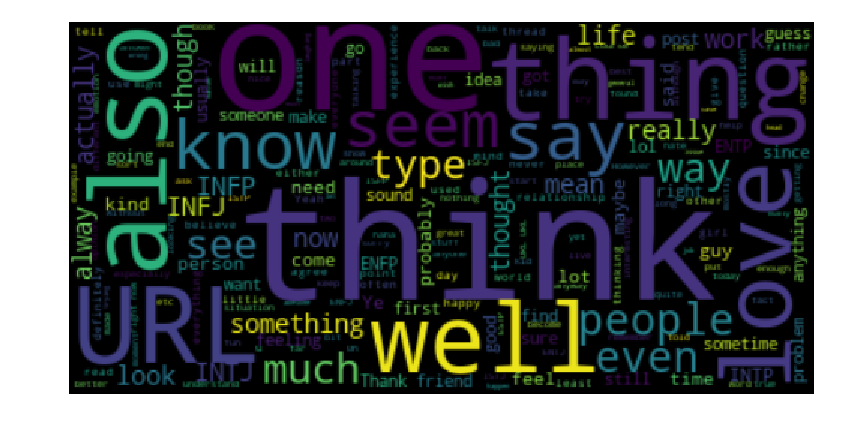
\includegraphics[scale=0.65]{wordclouds/wordcloud_all.pdf}
\end{figure}

\begin{figure}[htp] 
  \caption{word cloud generated from all documents with the ISTJ Myers-Briggs type indicator. As we can see, "ISTJ" is a common word for this subset of documents.}
  \label{fig:wordcloud-ISTJ}
  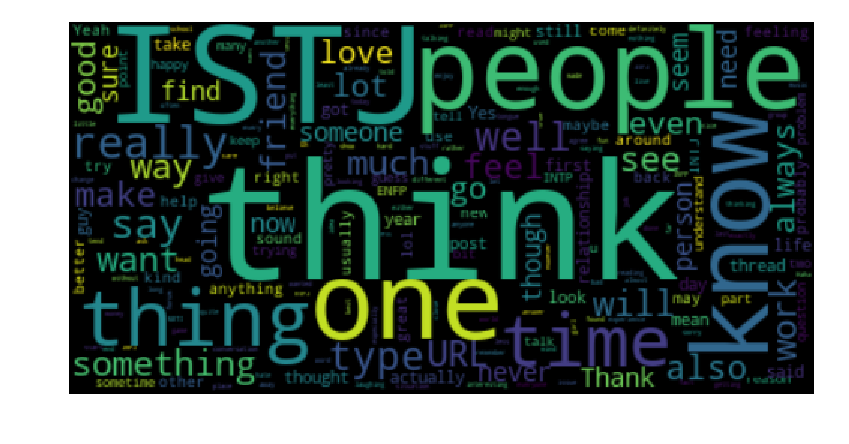
\includegraphics[scale=0.65]{wordclouds/wordcloud_ISTJ.pdf}
\end{figure}

\begin{figure}[htp] 
  \caption{word cloud generated from all documents with the ISFJ Myers-Briggs type indicator. As we can see, "ISFJ" is a common word for this subset of documents.}
  \label{fig:wordcloud-ISFJ}
  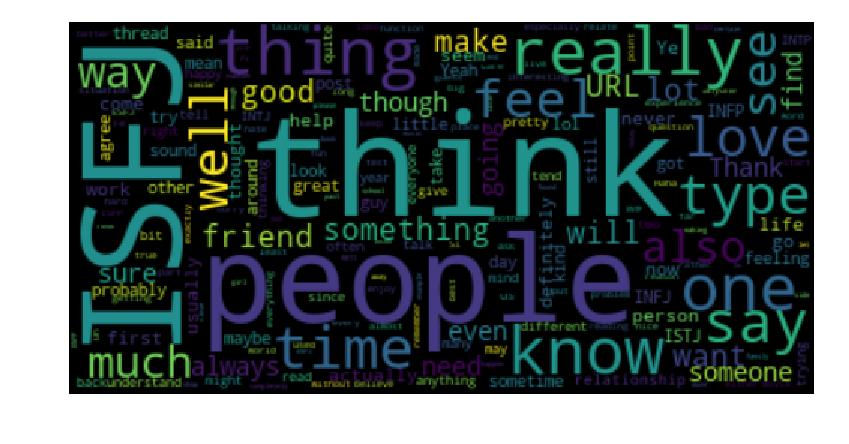
\includegraphics[scale=0.65]{wordclouds/wordcloud_ISFJ.pdf}
\end{figure}

\begin{figure}[htp] 
  \caption{word cloud generated from all documents with the INFJ Myers-Briggs type indicator. As we can see, "INFJ" is a common word for this subset of documents.}
  \label{fig:wordcloud-INFJ}
  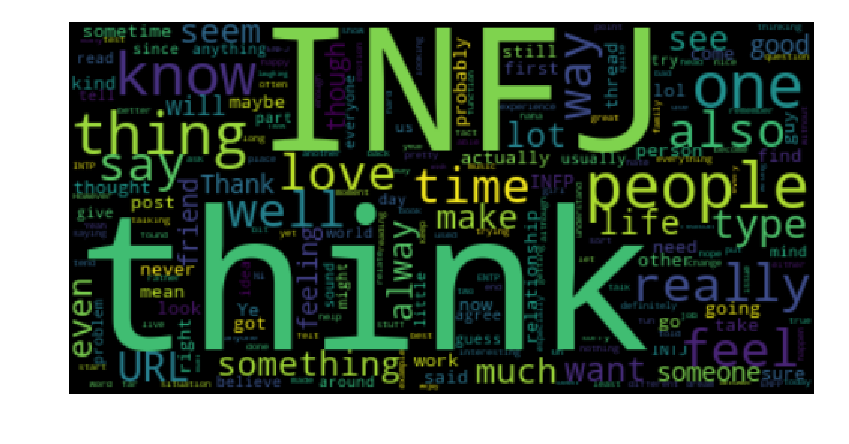
\includegraphics[scale=0.65]{wordclouds/wordcloud_INFJ.pdf}
\end{figure}

\begin{figure}[htp] 
  \caption{word cloud generated from all documents with the INTJ Myers-Briggs type indicator. As we can see, "INTJ" is a common word for this subset of documents.}
  \label{fig:wordcloud-INTJ}
  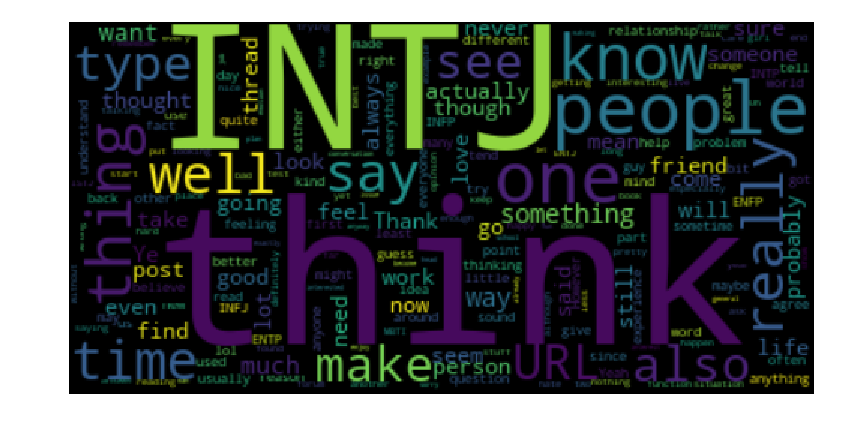
\includegraphics[scale=0.65]{wordclouds/wordcloud_INTJ.pdf}
\end{figure}

\begin{figure}[htp] 
  \caption{word cloud generated from all documents with the ISTP Myers-Briggs type indicator. As we can see, "ISTP" is a common word for this subset of documents.}
  \label{fig:wordcloud-ISTP}
  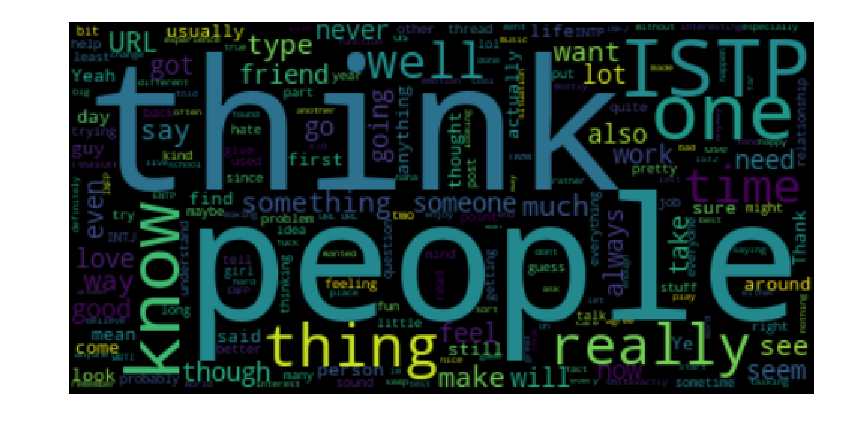
\includegraphics[scale=0.65]{wordclouds/wordcloud_ISTP.pdf}
\end{figure}

\begin{figure}[htp] 
  \caption{word cloud generated from all documents with the ISFP Myers-Briggs type indicator. As we can see, "ISFP" is a common word for this subset of documents.}
  \label{fig:wordcloud-ISFP}
  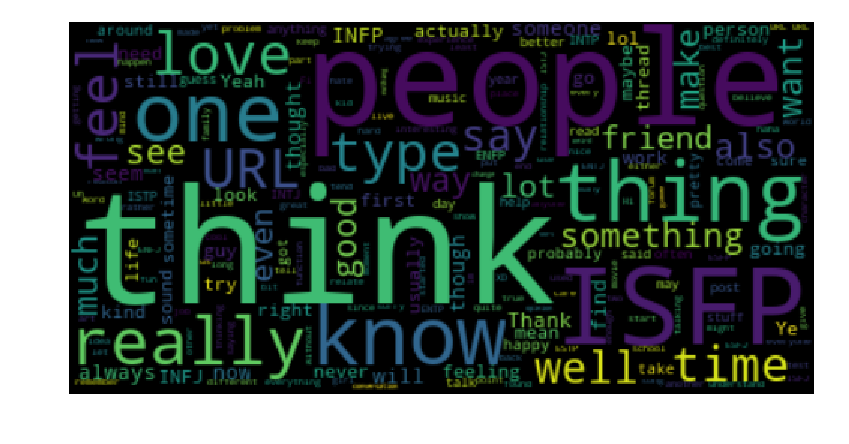
\includegraphics[scale=0.65]{wordclouds/wordcloud_ISFP.pdf}
\end{figure}

\begin{figure}[htp] 
  \caption{word cloud generated from all documents with the INFP Myers-Briggs type indicator. As we can see, "INFP" is a common word for this subset of documents.}
  \label{fig:wordcloud-INFP}
  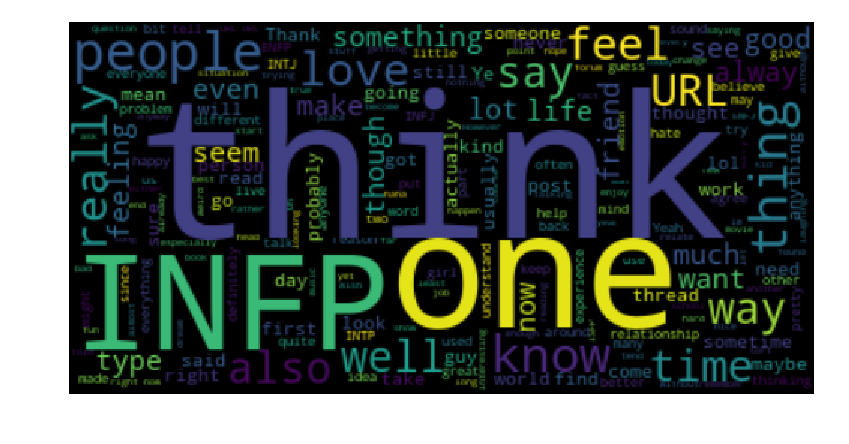
\includegraphics[scale=0.65]{wordclouds/wordcloud_INFP.pdf}
\end{figure}

\begin{figure}[htp] 
  \caption{word cloud generated from all documents with the INTP Myers-Briggs type indicator. As we can see, "INTP" is a common word for this subset of documents.}
  \label{fig:wordcloud-INTP}
  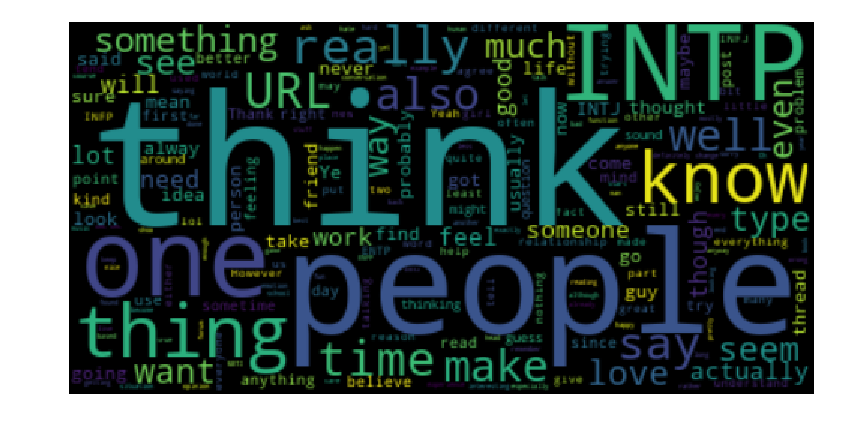
\includegraphics[scale=0.65]{wordclouds/wordcloud_INTP.pdf}
\end{figure}

\begin{figure}[htp] 
  \caption{word cloud generated from all documents with the ESTP Myers-Briggs type indicator. As we can see, "ESTP" is a common word for this subset of documents.}
  \label{fig:wordcloud-ESTP}
  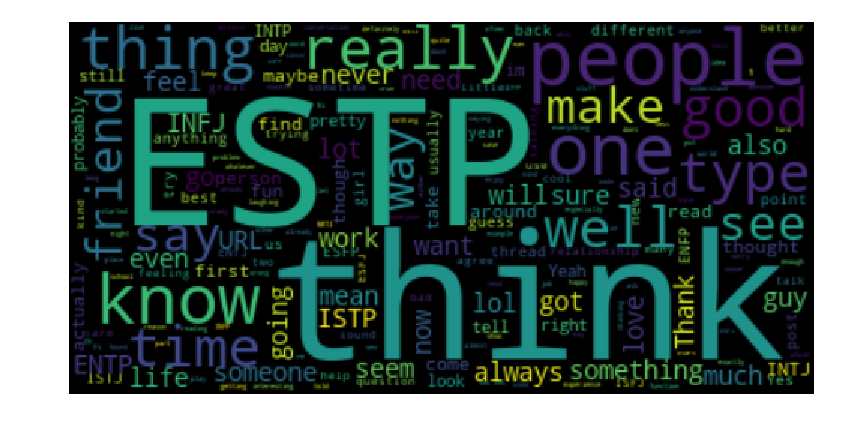
\includegraphics[scale=0.65]{wordclouds/wordcloud_ESTP.pdf}
\end{figure}

\begin{figure}[htp] 
  \caption{word cloud generated from all documents with the ESFP Myers-Briggs type indicator. As we can see, "ESFP" is a common word for this subset of documents.}
  \label{fig:wordcloud-ESFP}
  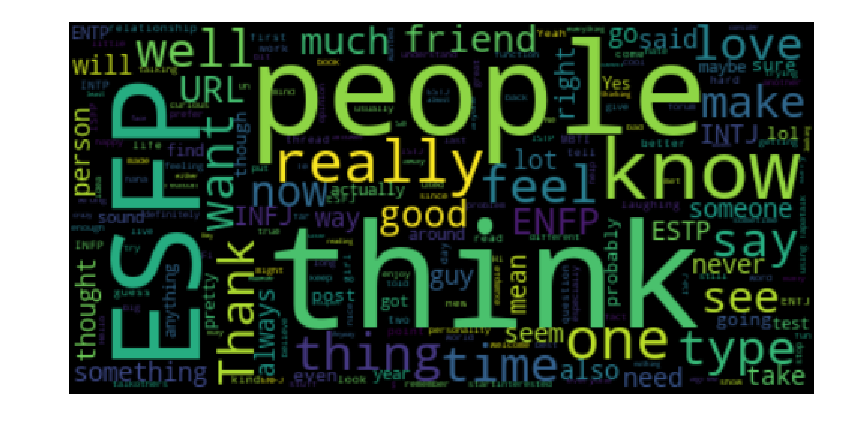
\includegraphics[scale=0.65]{wordclouds/wordcloud_ESFP.pdf}
\end{figure}

\begin{figure}[htp] 
  \caption{word cloud generated from all documents with the ENFP Myers-Briggs type indicator. As we can see, "ENFP" is a common word for this subset of documents.}
  \label{fig:wordcloud-ENFP}
  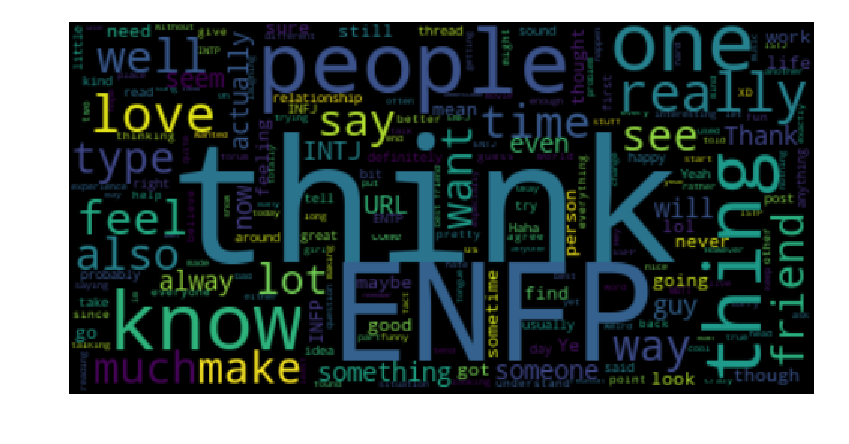
\includegraphics[scale=0.65]{wordclouds/wordcloud_ENFP.pdf}
\end{figure}

\begin{figure}[htp] 
  \caption{word cloud generated from all documents with the ENTP Myers-Briggs type indicator. As we can see, "ENTP" is a common word for this subset of documents.}
  \label{fig:wordcloud-ENTP}
  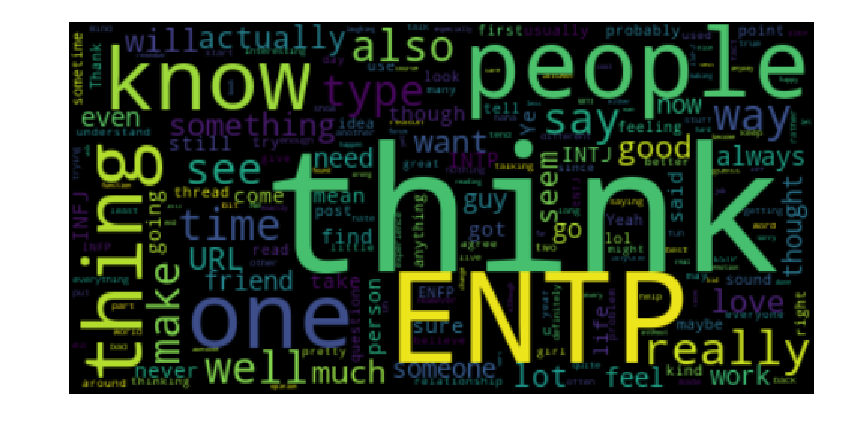
\includegraphics[scale=0.65]{wordclouds/wordcloud_ENTP.pdf}
\end{figure}

\begin{figure}[htp] 
  \caption{word cloud generated from all documents with the ESTJ Myers-Briggs type indicator. As we can see, "ESTJ" is a common word for this subset of documents.}
  \label{fig:wordcloud-ESTJ}
  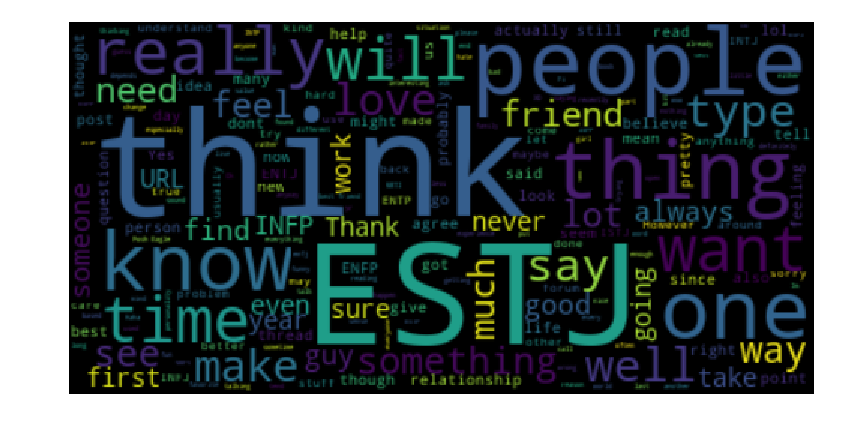
\includegraphics[scale=0.65]{wordclouds/wordcloud_ESTJ.pdf}
\end{figure}

\begin{figure}[htp] 
  \caption{word cloud generated from all documents with the ESFJ Myers-Briggs type indicator. As we can see, "ESFJ" is a common word for this subset of documents.}
  \label{fig:wordcloud-ESFJ}
  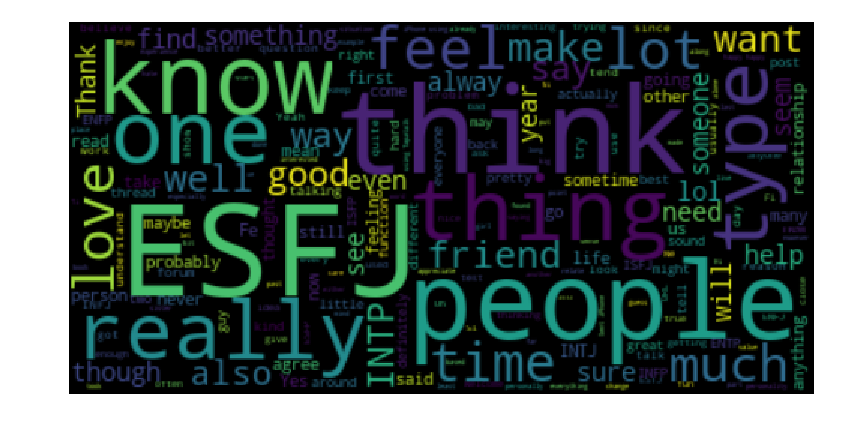
\includegraphics[scale=0.65]{wordclouds/wordcloud_ESFJ.pdf}
\end{figure}

\begin{figure}[htp] 
  \caption{word cloud generated from all documents with the ENFJ Myers-Briggs type indicator. As we can see, "ENFJ" is a common word for this subset of documents.}
  \label{fig:wordcloud-ENFJ}
  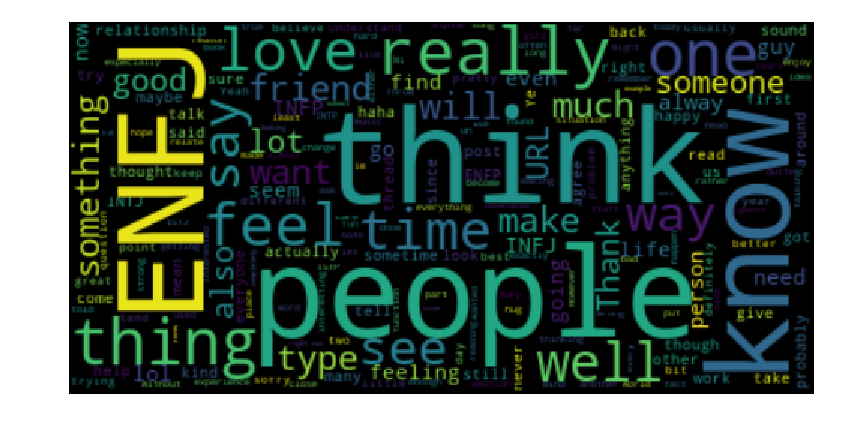
\includegraphics[scale=0.65]{wordclouds/wordcloud_ENFJ.pdf}
\end{figure}

\begin{figure}[htp] 
  \caption{word cloud generated from all documents with the ENTJ Myers-Briggs type indicator. As we can see, "ENTJ" is a common word for this subset of documents.}
  \label{fig:wordcloud-ENTJ}
  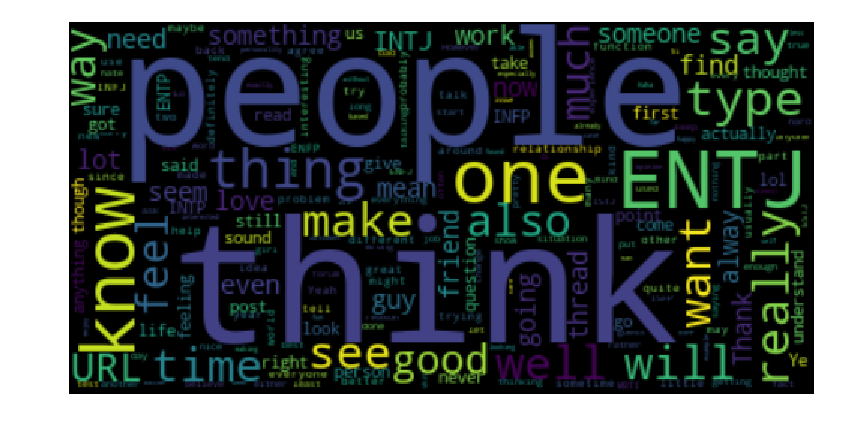
\includegraphics[scale=0.65]{wordclouds/wordcloud_ENTJ.pdf}
\end{figure}

%
%Some text for the appendix.

% use section* for acknowledgement
%\section*{Acknowledgment}


%The authors would like to thank...


% Can use something like this to put references on a page
% by themselves when using endfloat and the captionsoff option.
\ifCLASSOPTIONcaptionsoff
  \newpage
\fi



% trigger a \newpage just before the given reference
% number - used to balance the columns on the last page
% adjust value as needed - may need to be readjusted if
% the document is modified later
%\IEEEtriggeratref{8}
% The "triggered" command can be changed if desired:
%\IEEEtriggercmd{\enlargethispage{-5in}}

% references section

% can use a bibliography generated by BibTeX as a .bbl file
% BibTeX documentation can be easily obtained at:
% http://www.ctan.org/tex-archive/biblio/bibtex/contrib/doc/
% The IEEEtran BibTeX style support page is at:
% http://www.michaelshell.org/tex/ieeetran/bibtex/

% argument is your BibTeX string definitions and bibliography database(s)
%\bibliography{IEEEabrv,../bib/paper}
%
% <OR> manually copy in the resultant .bbl file
% set second argument of \begin to the number of references
% (used to reserve space for the reference number labels box)
%\begin{thebibliography}{1}

%\bibitem{IEEEhowto:kopka}
%H.~Kopka and P.~W. Daly, \emph{A Guide to \LaTeX}, 3rd~ed.\hskip 1em plus
%  0.5em minus 0.4em\relax Harlow, England: Addison-Wesley, 1999.

%\end{thebibliography}

% biography section
% 
% If you have an EPS/PDF photo (graphicx package needed) extra braces are
% needed around the contents of the optional argument to biography to prevent
% the LaTeX parser from getting confused when it sees the complicated
% \includegraphics command within an optional argument. (You could create
% your own custom macro containing the \includegraphics command to make things
% simpler here.)
%\begin{biography}[{\includegraphics[width=1in,height=1.25in,clip,keepaspectratio]{mshell}}]{Michael Shell}
% or if you just want to reserve a space for a photo:

%\begin{IEEEbiography}[{
\includegraphics[width=1in,height=1.25in,clip,keepaspectratio]{picture}}]{John Doe}
%\blindtext
%\end{IEEEbiography}

% You can push biographies down or up by placing
% a \vfill before or after them. The appropriate
% use of \vfill depends on what kind of text is
% on the last page and whether or not the columns
% are being equalized.

%\vfill

% Can be used to pull up biographies so that the bottom of the last one
% is flush with the other column.
%\enlargethispage{-5in}



% that's all folks
\end{document}


